\documentclass{article}
\usepackage{graphicx} 

\setlength{\parindent}{15pt}
\setlength{\parskip}{5pt}

\usepackage[margin=0.75in]{geometry}
\usepackage{amssymb}
\usepackage{amsmath}
\usepackage{mathtools}
\usepackage{xcolor}
\usepackage{cancel}
\usepackage{centernot}
\usepackage{nicefrac}
\usepackage{bm}
\usepackage{indentfirst}
\usepackage{float}
\usepackage[round]{natbib} 
\usepackage[hidelinks]{hyperref}
\usepackage{enumerate}
\usepackage{titling}
\usepackage{enumitem}
\usepackage{parskip}
\usepackage{subcaption}

\setlist[itemize]{label=\textendash}

\newenvironment{answer}{\par\vspace{0.8em}\textbf{A:}}{\par}
\newcommand{\red}[1]{\textcolor{red}{#1}}
\newcommand{\blue}[1]{\textcolor{blue}{#1}}
\newcommand{\fa}{\text{ for all }} 
\newcommand{\ex}{\text{ there exists }}
\newcommand{\st}{\text{ such that }}
\newcommand{\for}{\text{ for }}
\newcommand{\andt}{\text{ and }}
\newcommand{\ort}{\text{ or }}
\newcommand{\ift}{\text{ if }}
\newcommand{\where}{\text{ where }}
\newcommand{\but}{\text{ but }}
\newcommand{\nat}{\mathbb{N}}
\newcommand{\rat}{\mathbb{Q}}
\newcommand{\com}{\mathbb{C}}
\newcommand{\real}{\mathbb{R}}
\newcommand{\norm}[1]{\lVert#1\rVert}
\newcommand{\abs}[1]{\lvert#1\rvert}
\newcommand{\corr}{\rightrightarrows}
\newcommand{\ul}{\underline}
\newcommand{\bft}{\textbf}
\newcommand{\itt}{\textit}
\newcommand{\E}{\mathbb{E}}
\newcommand{\Prob}{\operatorname{P}}
\newcommand{\Var}{\operatorname{Var}}
\newcommand{\Cov}{\operatorname{Cov}}
\newcommand{\Unif}{\operatorname{Unif}}
\newcommand{\Bias}{\operatorname{Bias}}
\newcommand{\N}{\operatorname{N}}
\newcommand{\MSE}{\operatorname{MSE}}
\newcommand{\iffs}{\Leftrightarrow}
\newcommand{\prefeq}{\trianglerighteq}
\newcommand{\pref}{\triangleright}
\newcommand{\indiff}{\mathrel{\triangleright\triangleleft}}

\title{Age gradient graphs}
\date{\today}

\begin{document}

\maketitle

% \section*{\centering \LARGE \normalfont Current evidence}

\section*{Longitudinal age trend}



\begin{figure}[H]
    \centering
    \caption{Selected longitudinal questions}
    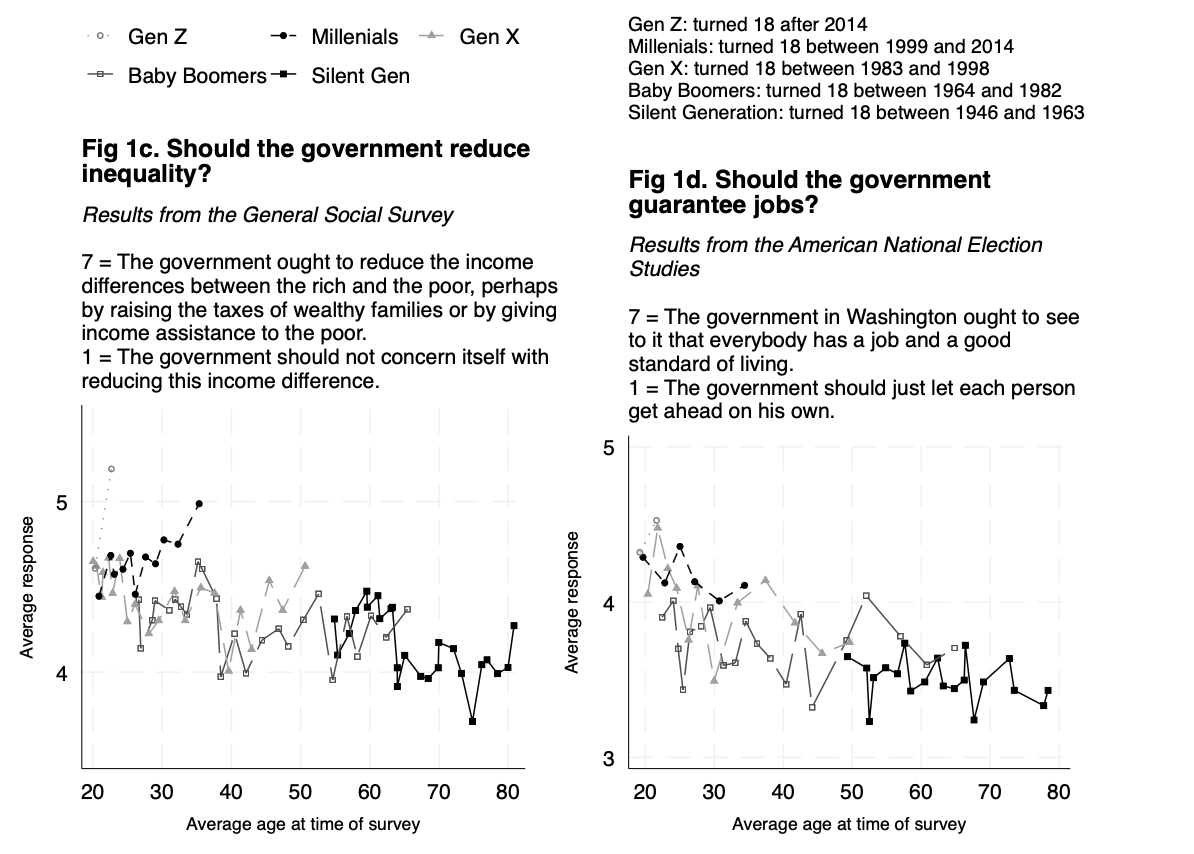
\includegraphics[width=.75\linewidth]{images/long_age.png}
\end{figure}
\begin{figure}[H]
    \centering
    \caption{Other longitudinal questions}
    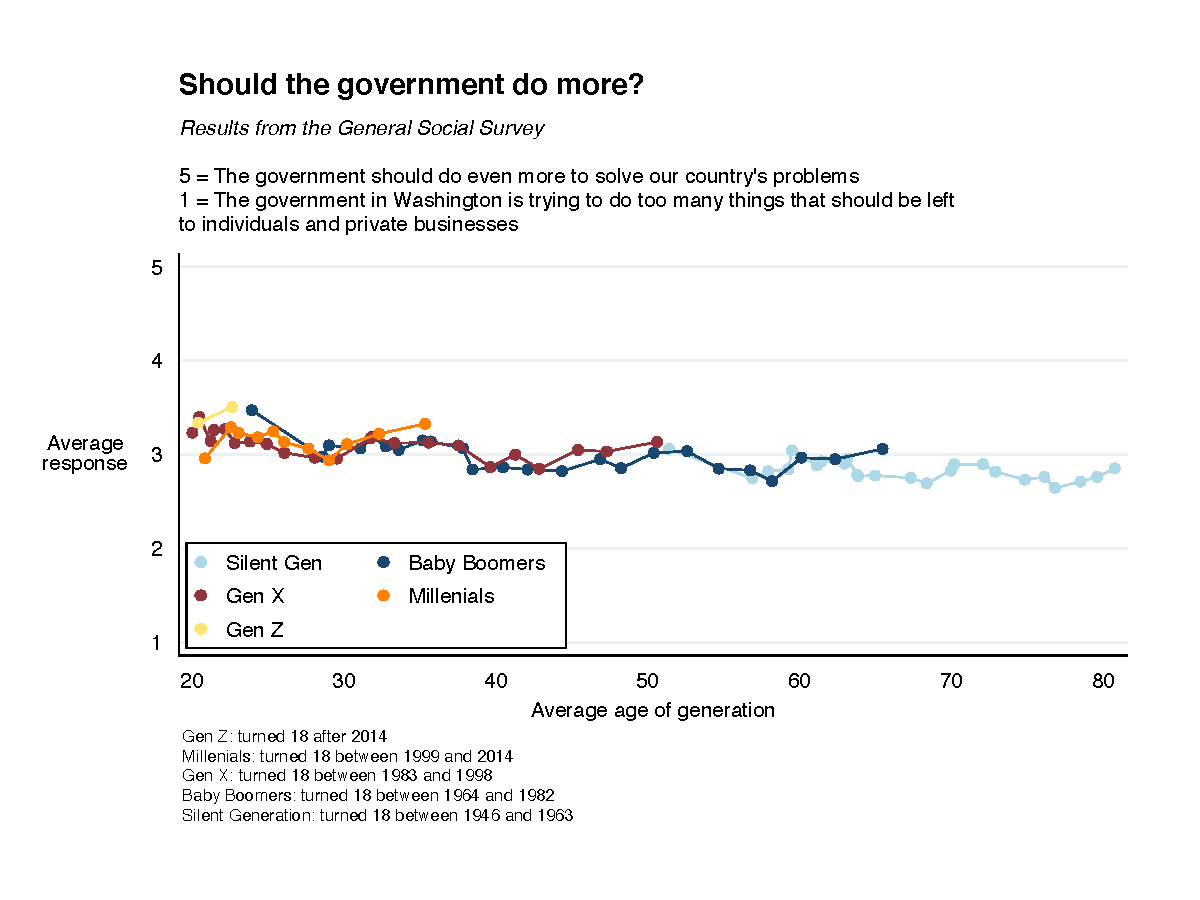
\includegraphics[width=.8\linewidth]{images/gss_domore.pdf}
\end{figure}
\begin{figure}[H]
    \centering
    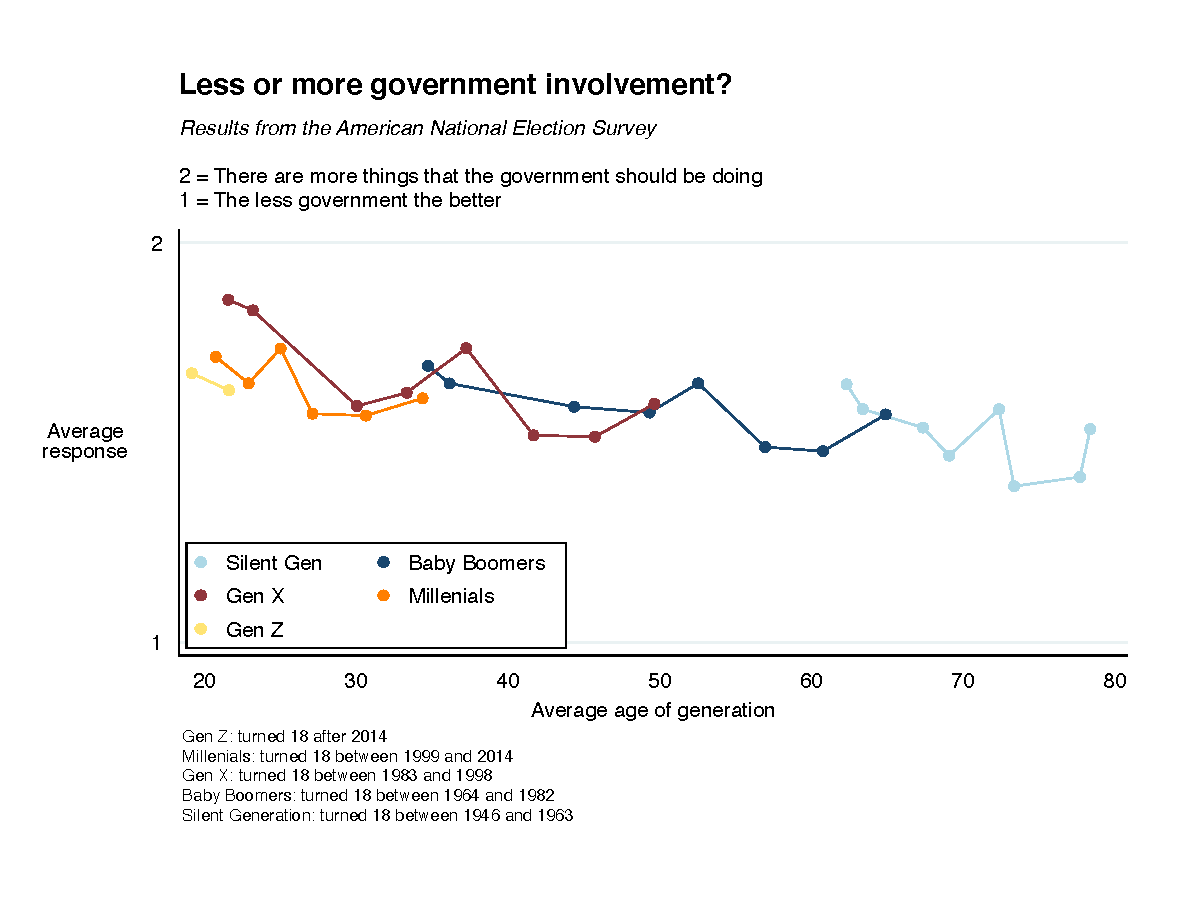
\includegraphics[width=.8\linewidth]{images/anes_involvement.pdf}
\end{figure}

\begin{figure}[H]
    \centering
    \caption{GSS ``should government reduce inequality'' cohort gradients}
    \begin{subfigure}{.49\textwidth}
        \centering
        \caption{Without generation fixed effects}
        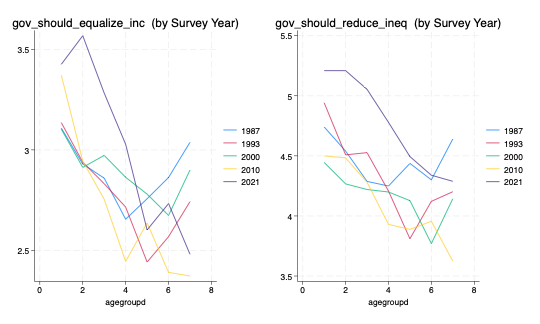
\includegraphics[width=\linewidth]{images/gen_fe_gss.png}
    \end{subfigure}
    \begin{subfigure}{.49\textwidth}
        \centering
        \caption{With generation fixed effects}
        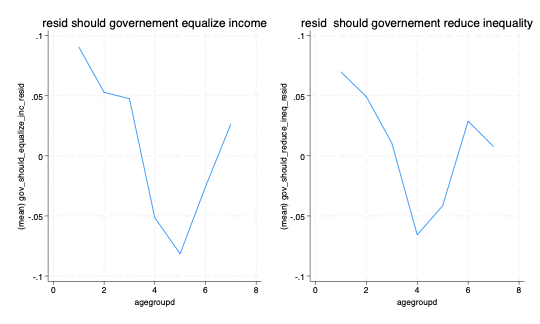
\includegraphics[width=\linewidth]{images/gen_fe.png}
    \end{subfigure}
\end{figure}

\begin{figure}[H]
    \centering
    \caption{WVS cohort gradients}
    \begin{subfigure}{.49\textwidth}
        \centering
        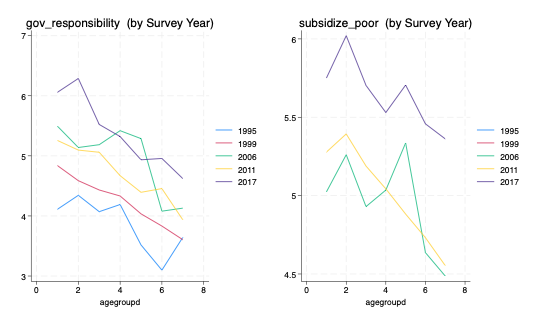
\includegraphics[width=\linewidth]{images/wvs_nofe1.png}
    \end{subfigure}
    \begin{subfigure}{.49\textwidth}
        \centering
        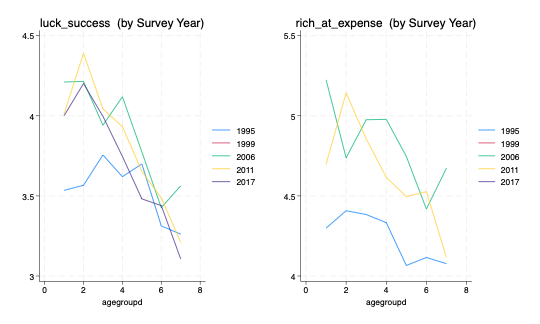
\includegraphics[width=\linewidth]{images/wvs_nofe2.png}
    \end{subfigure}
\end{figure}

% \begin{figure}[H]
%     \centering
%     \caption{GSS without generation fixed effects}
%     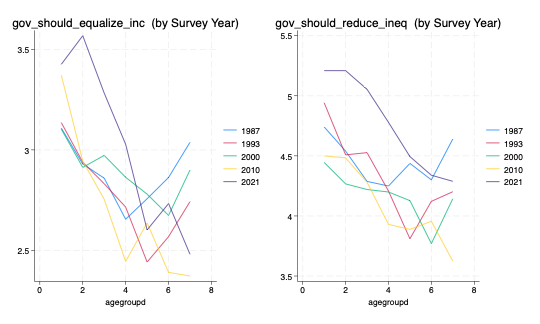
\includegraphics[width=.7\linewidth]{images/gen_fe_gss.png}
% \end{figure}
% \begin{figure}[H]
%     \centering
%     \caption{GSS with generation fixed effects}
%     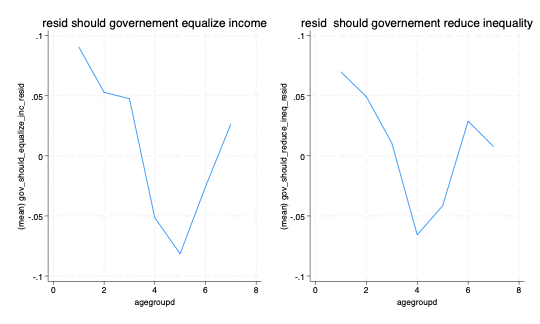
\includegraphics[width=.7\linewidth]{images/gen_fe.png}
% \end{figure}

\begin{figure}[H]
    \centering
    \caption{GSS ``government responsibility'' unadjusted age trends (Kodira)}
    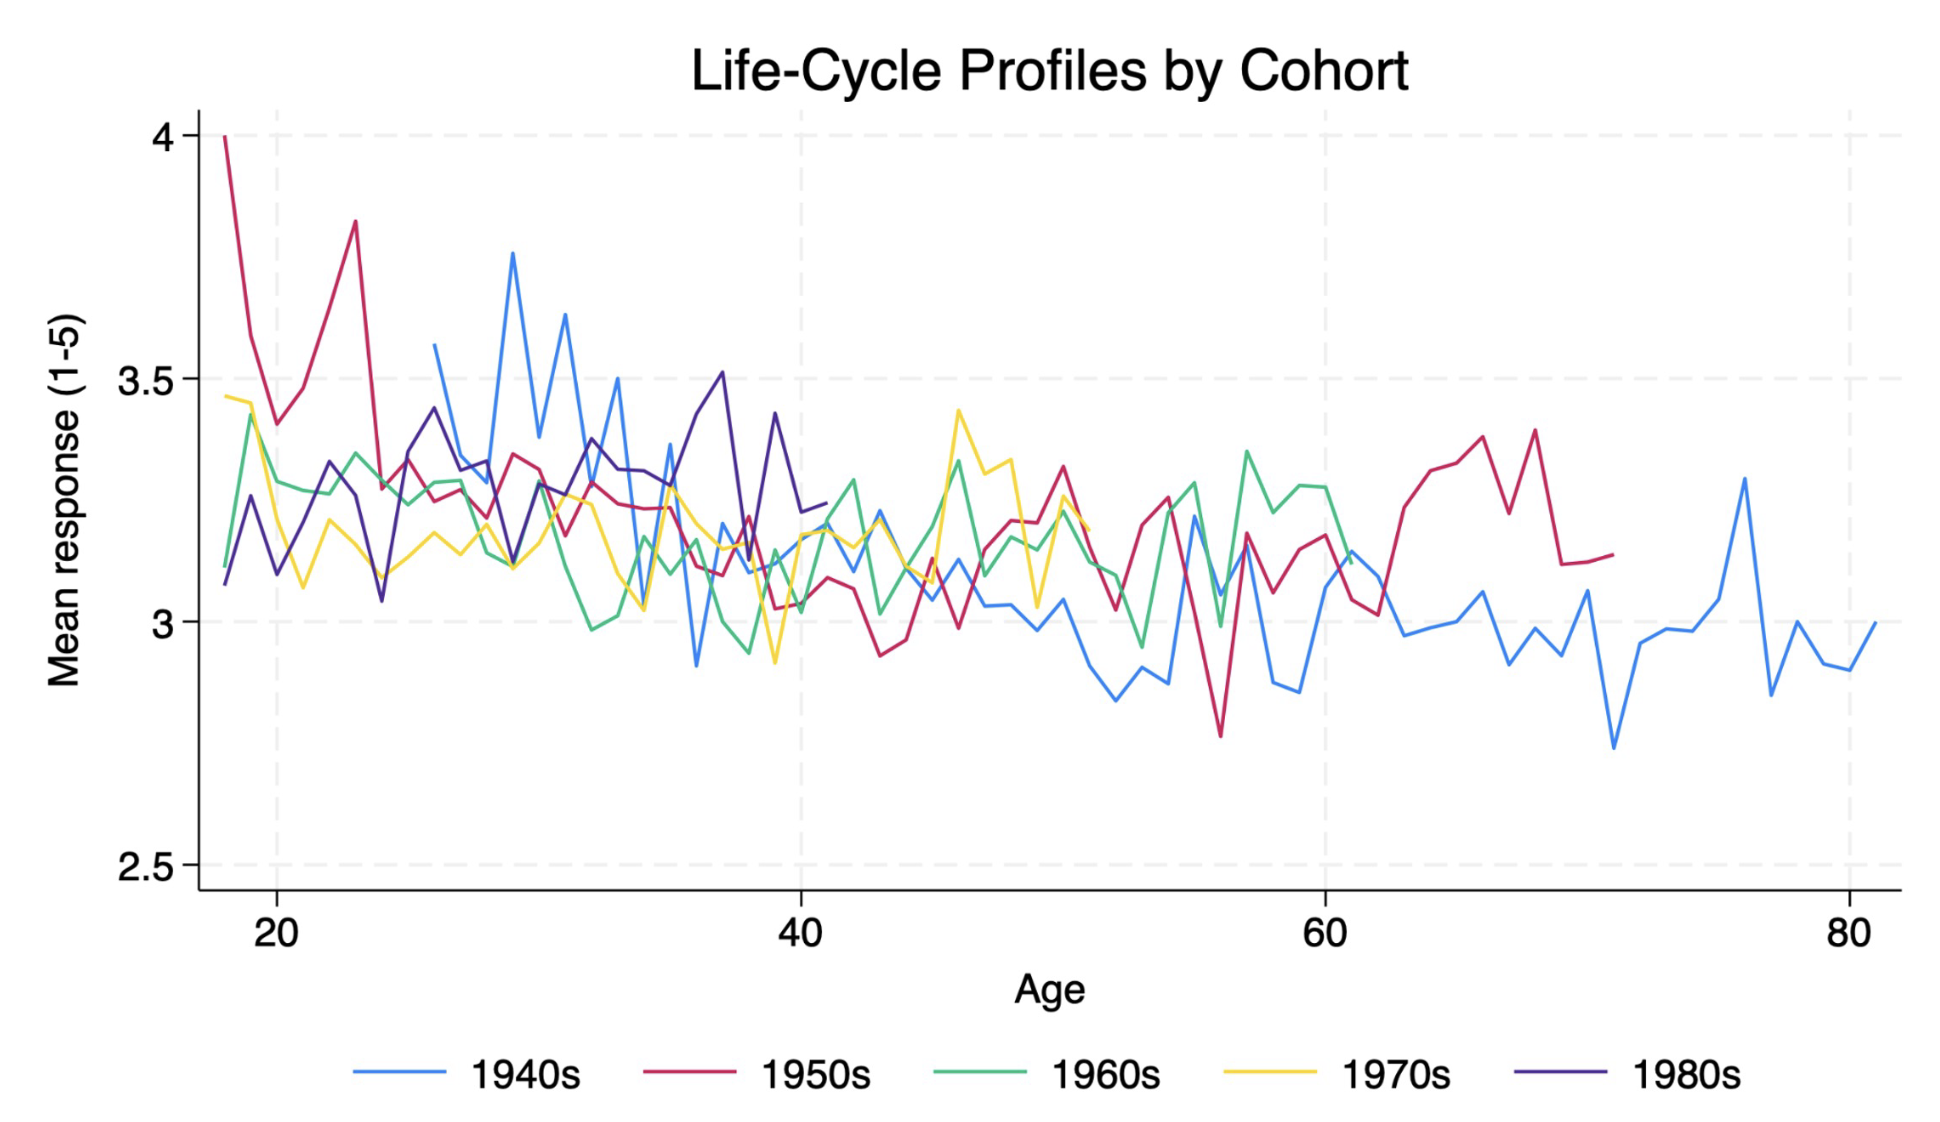
\includegraphics[width=.7\linewidth]{images/kodira_age.png}
\end{figure}

\begin{figure}[H]
    \centering
    \caption{Selected standard error bar graphs}
    \begin{subfigure}{.49\textwidth}
        \centering
        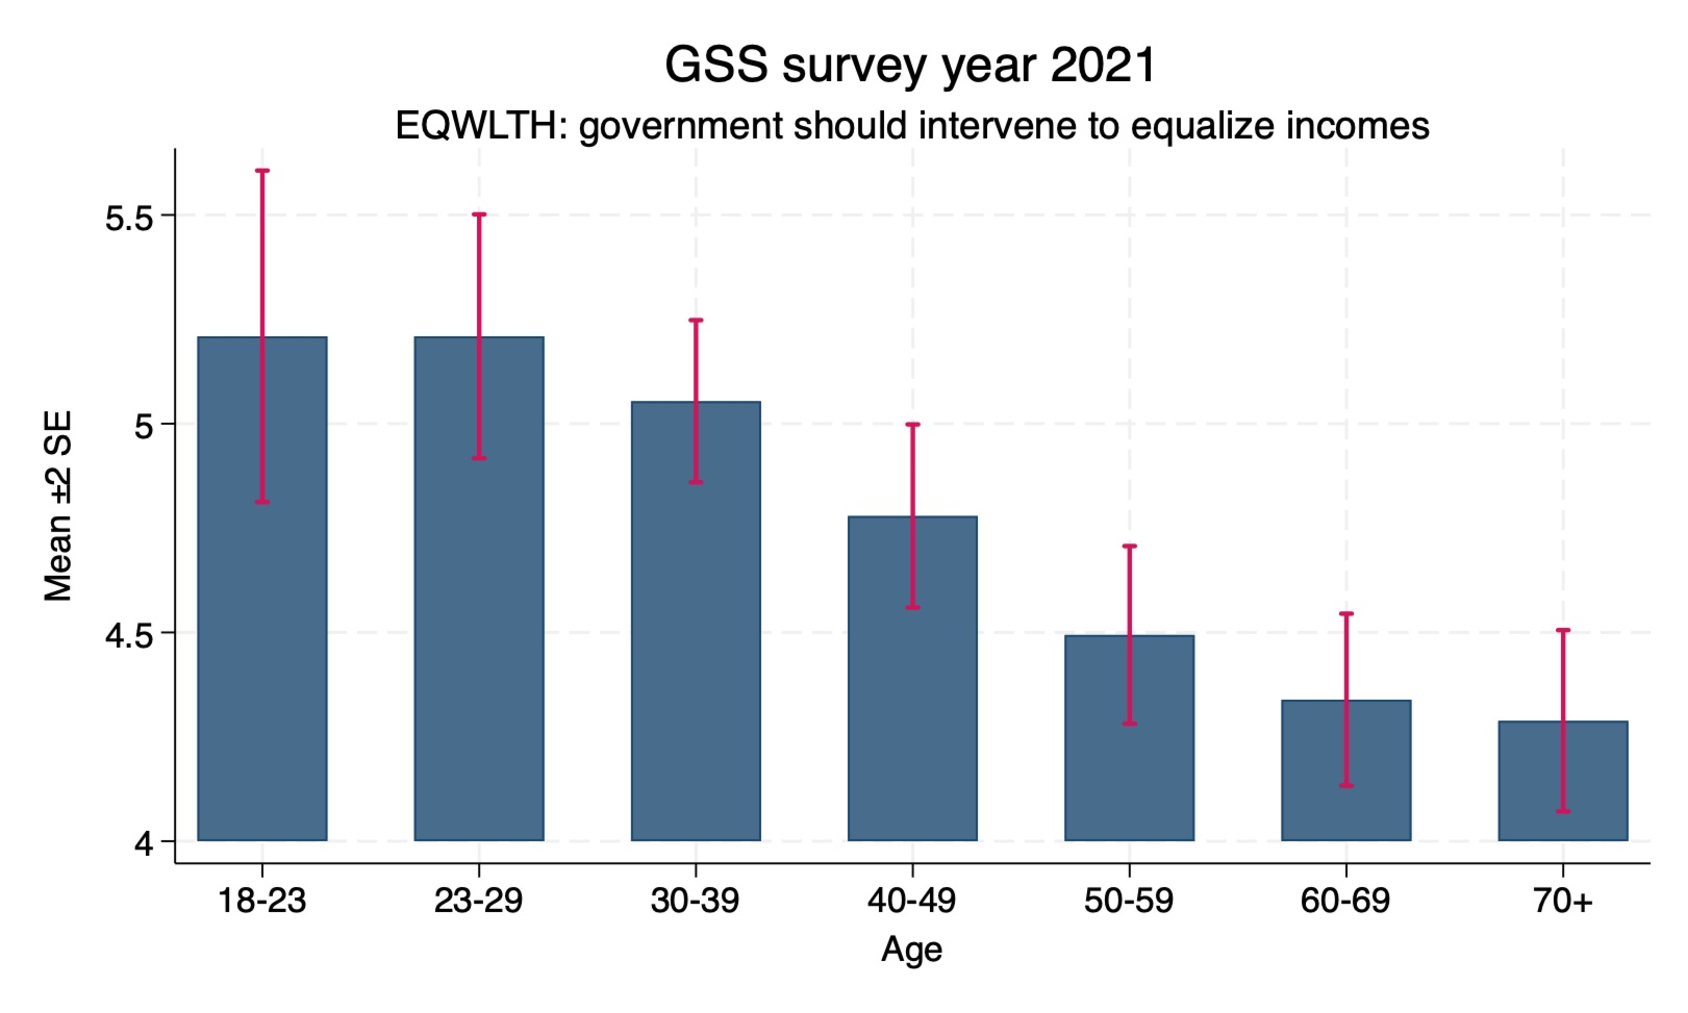
\includegraphics[width=\linewidth]{images/sebars_equalize2021.pdf}
    \end{subfigure}
    \begin{subfigure}{.49\textwidth}
        \centering
        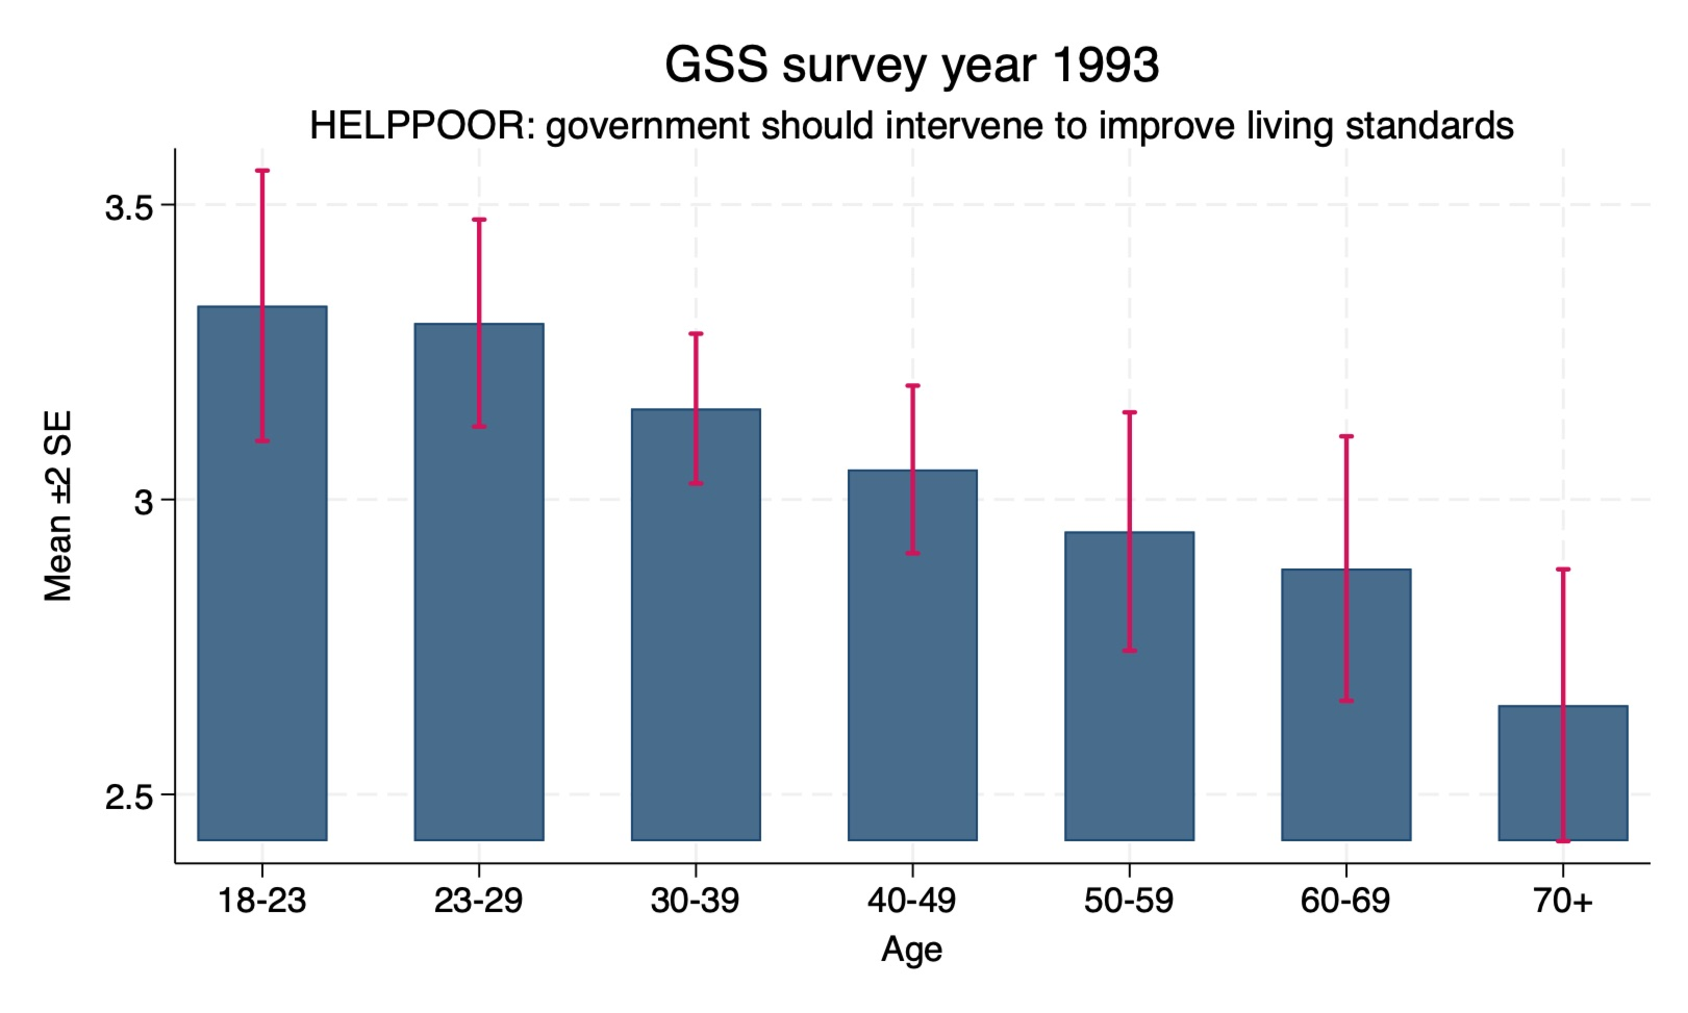
\includegraphics[width=\linewidth]{images/sebars_standards1993.pdf}
    \end{subfigure}
\end{figure}

\begin{figure}[H]
    \centering
    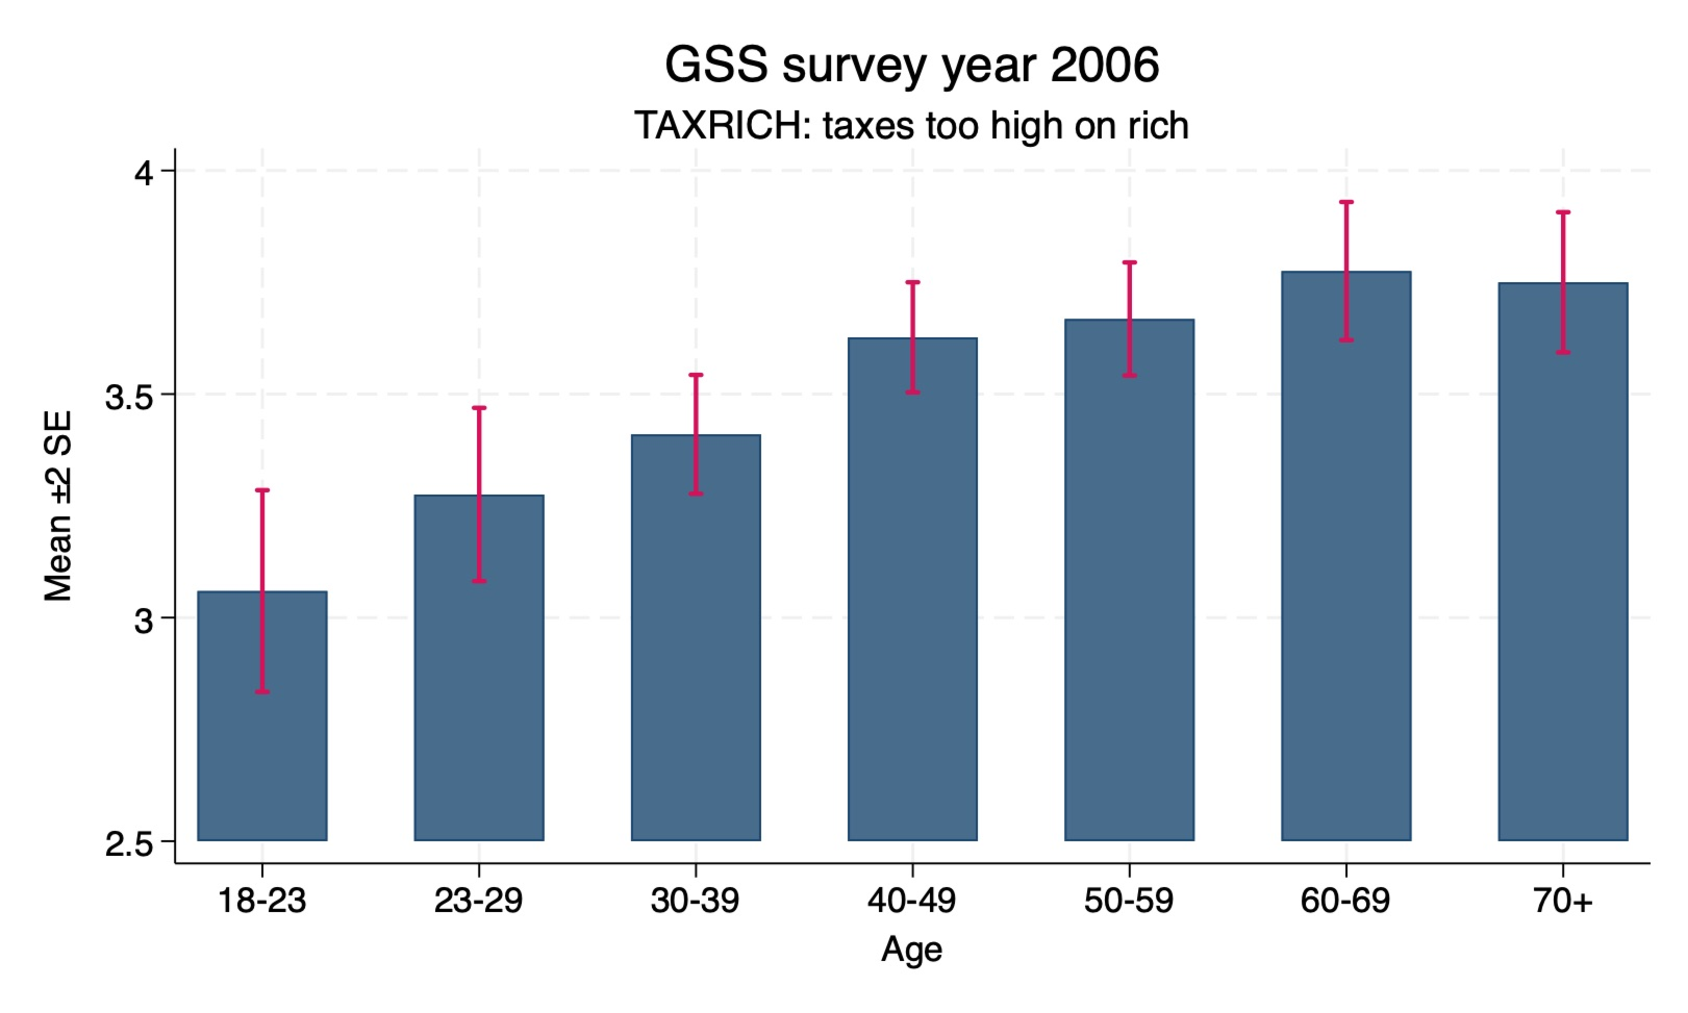
\includegraphics[width=.45\linewidth]{images/sebars_taxrich2006.pdf}
\end{figure}

% \begin{figure}[H]
%     \centering
%     \caption{Selected standard error bar graphs}
%     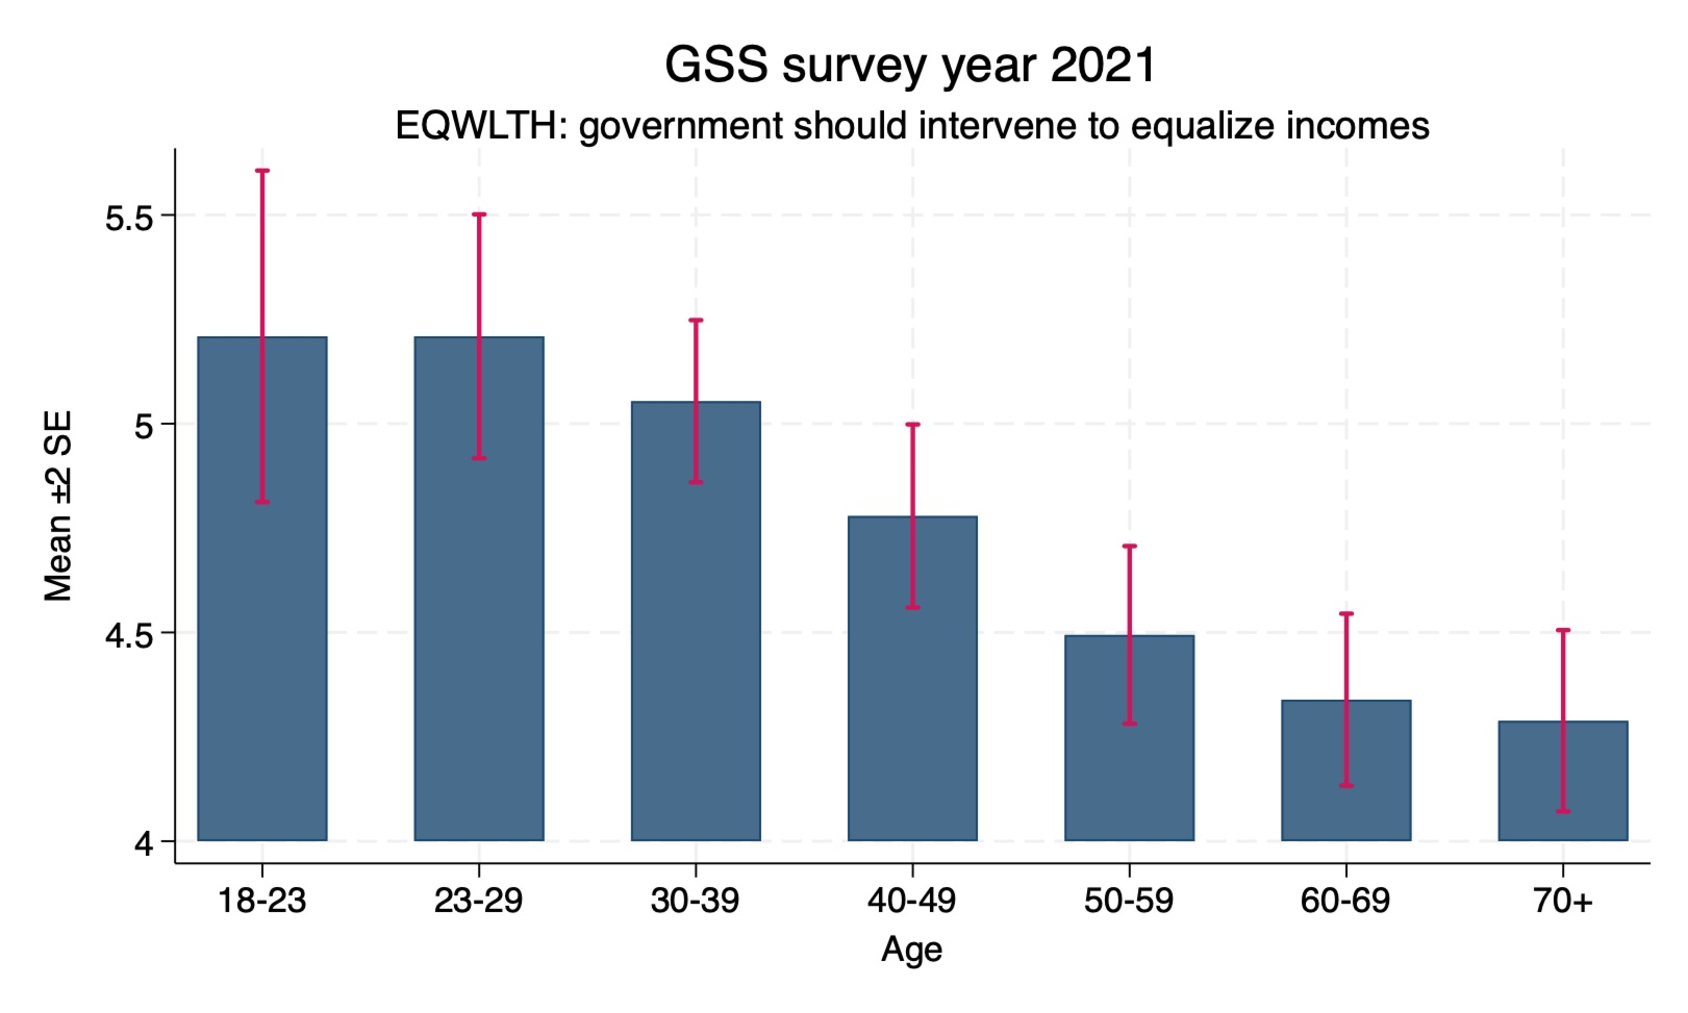
\includegraphics[width=.8\linewidth]{images/sebars_equalize2021.pdf}
% \end{figure}
% \begin{figure}[H]
%     \centering
%     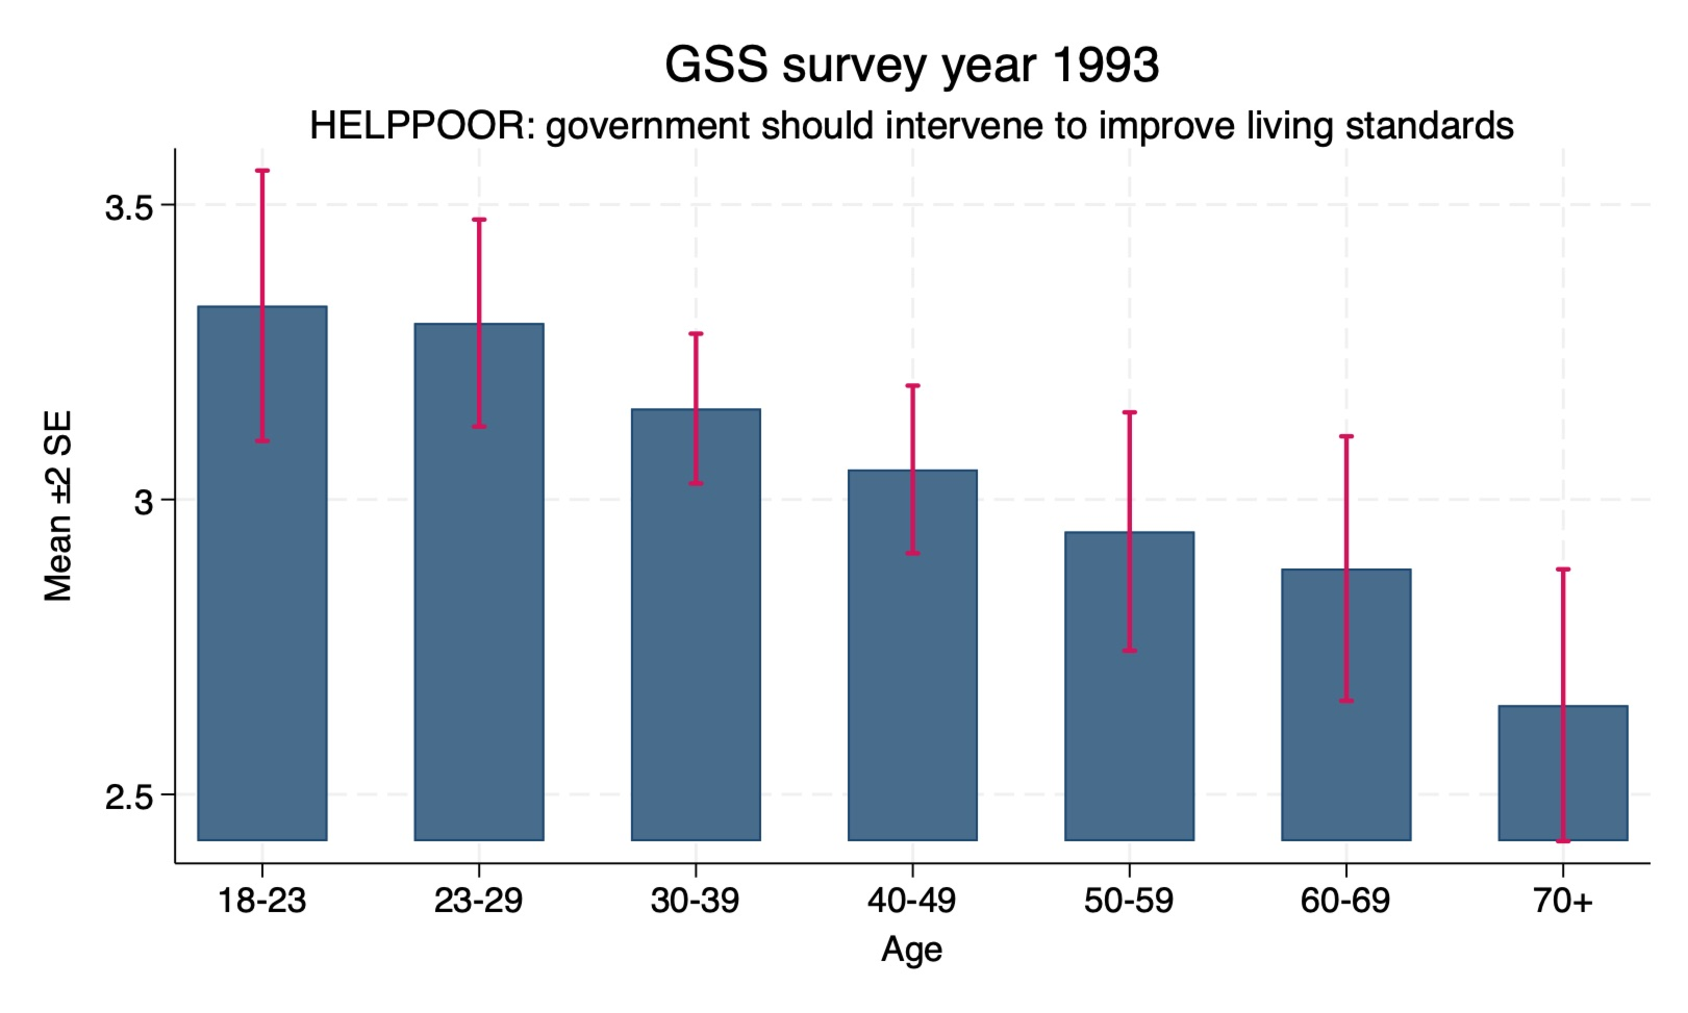
\includegraphics[width=.95\linewidth]{images/sebars_standards1993.pdf}
% \end{figure}
% \begin{figure}[H]
%     \centering
%     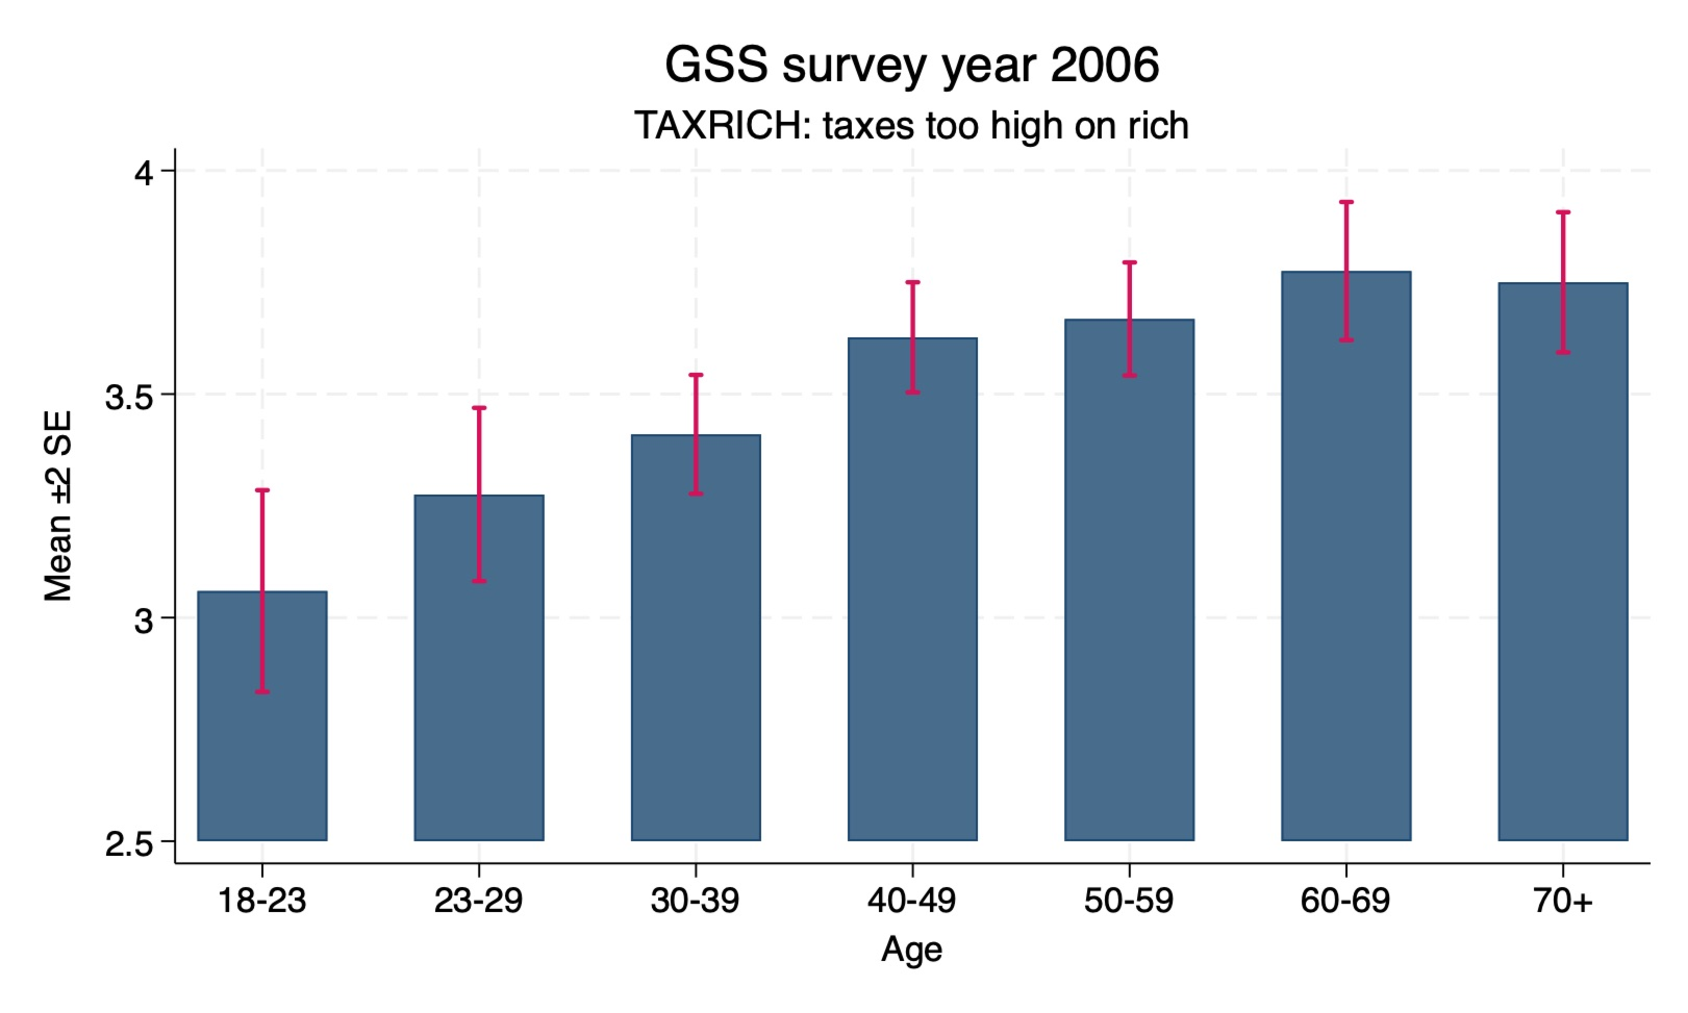
\includegraphics[width=.95\linewidth]{images/sebars_taxrich2006.pdf}
% \end{figure}

% \begin{figure}[H]
%     \centering
%     \begin{subfigure}[H]{\textwidth}
%         \centering
%         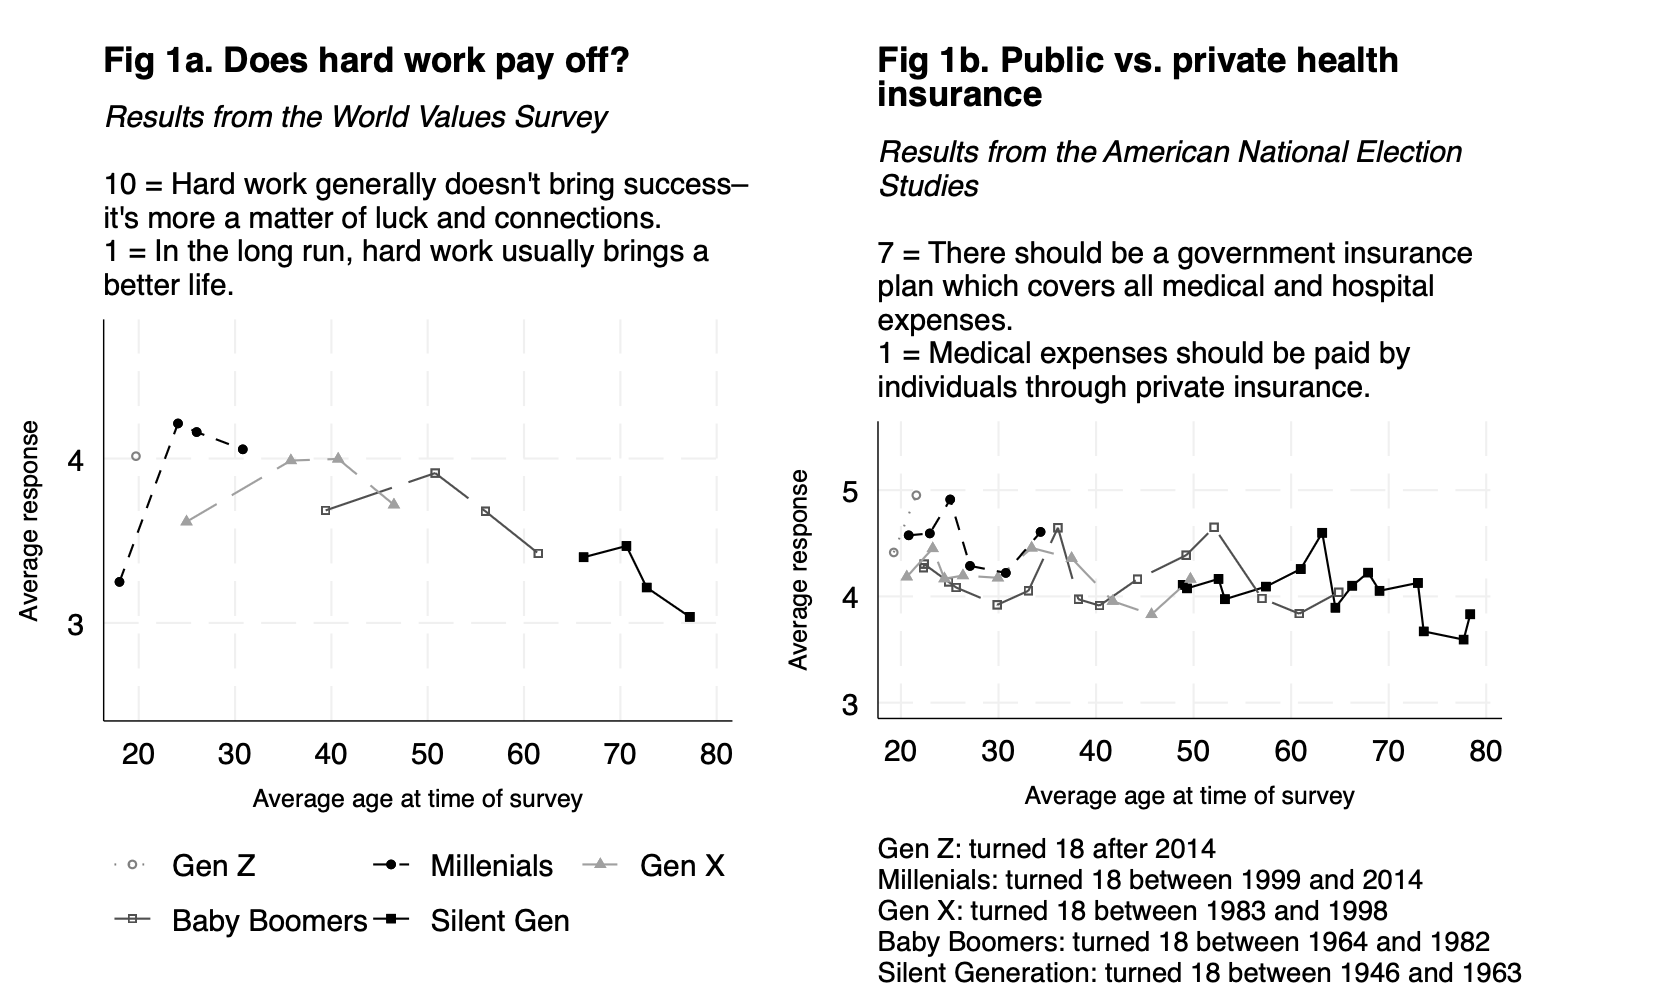
\includegraphics[width=\linewidth]{images/long_age1.png}
%     \end{subfigure}
%     \begin{subfigure}{\textwidth}
%         \centering
%         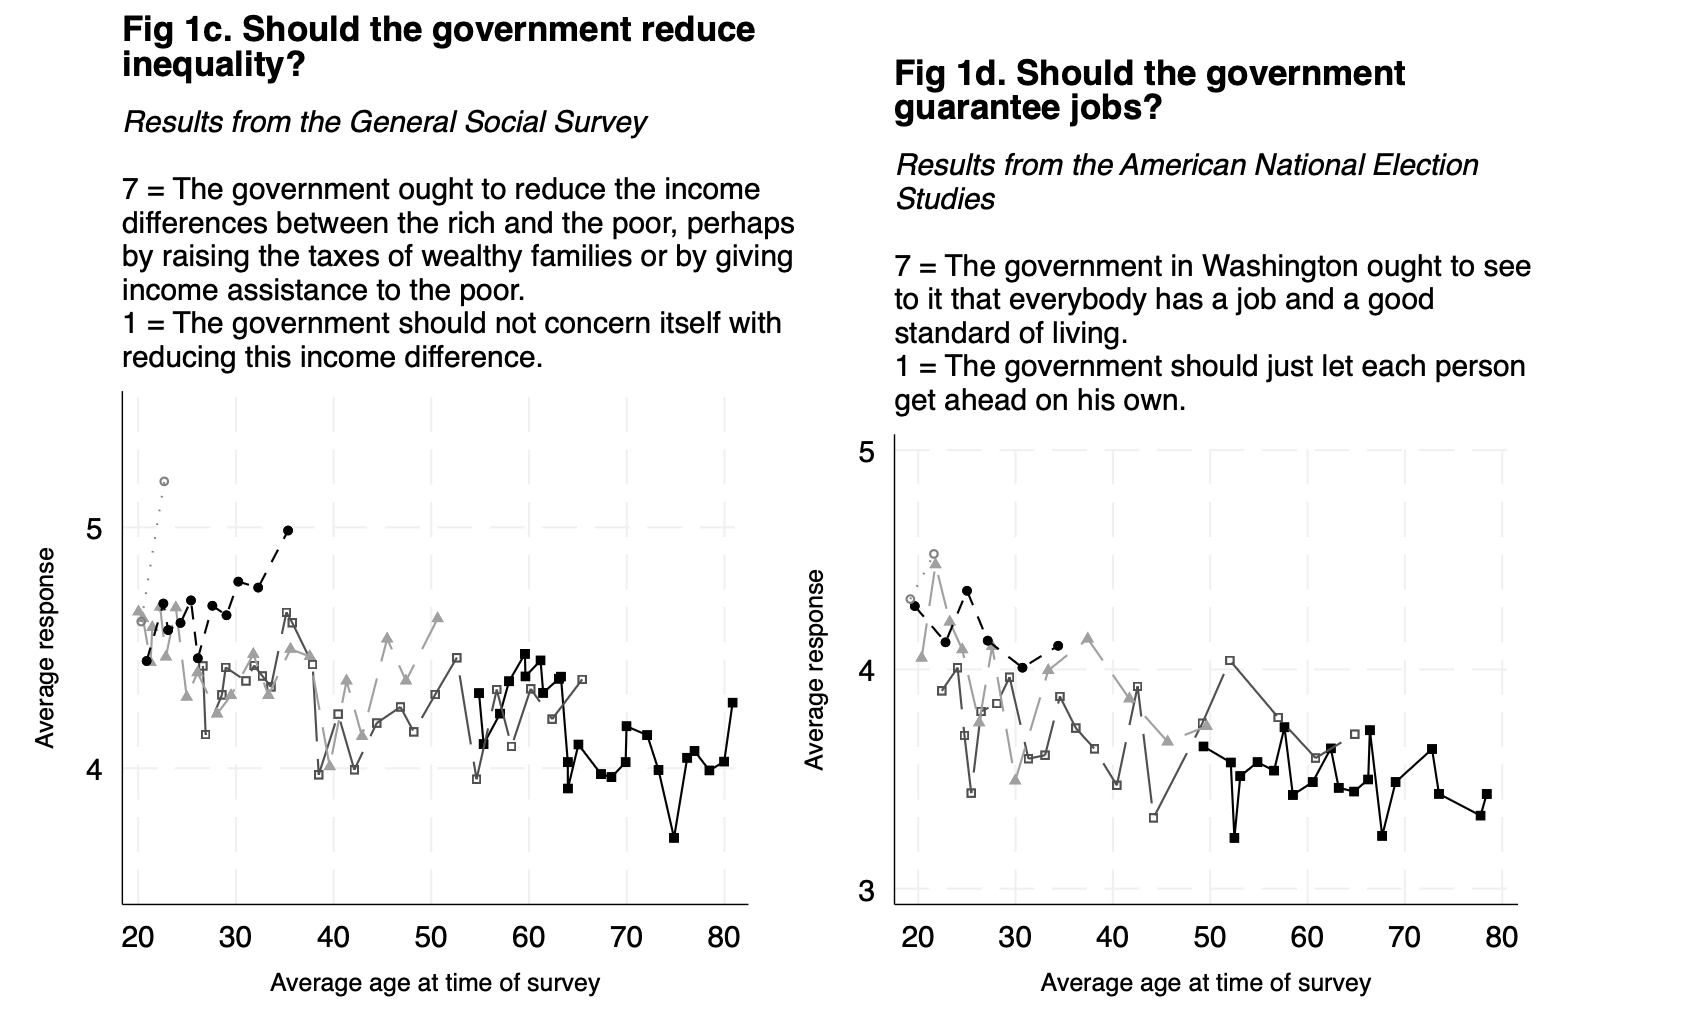
\includegraphics[width=\linewidth]{images/long_age2.png}
%     \end{subfigure}
%     \label{fig:long-age}
% \end{figure}
% \begin{figure}[H]
%     \centering
%     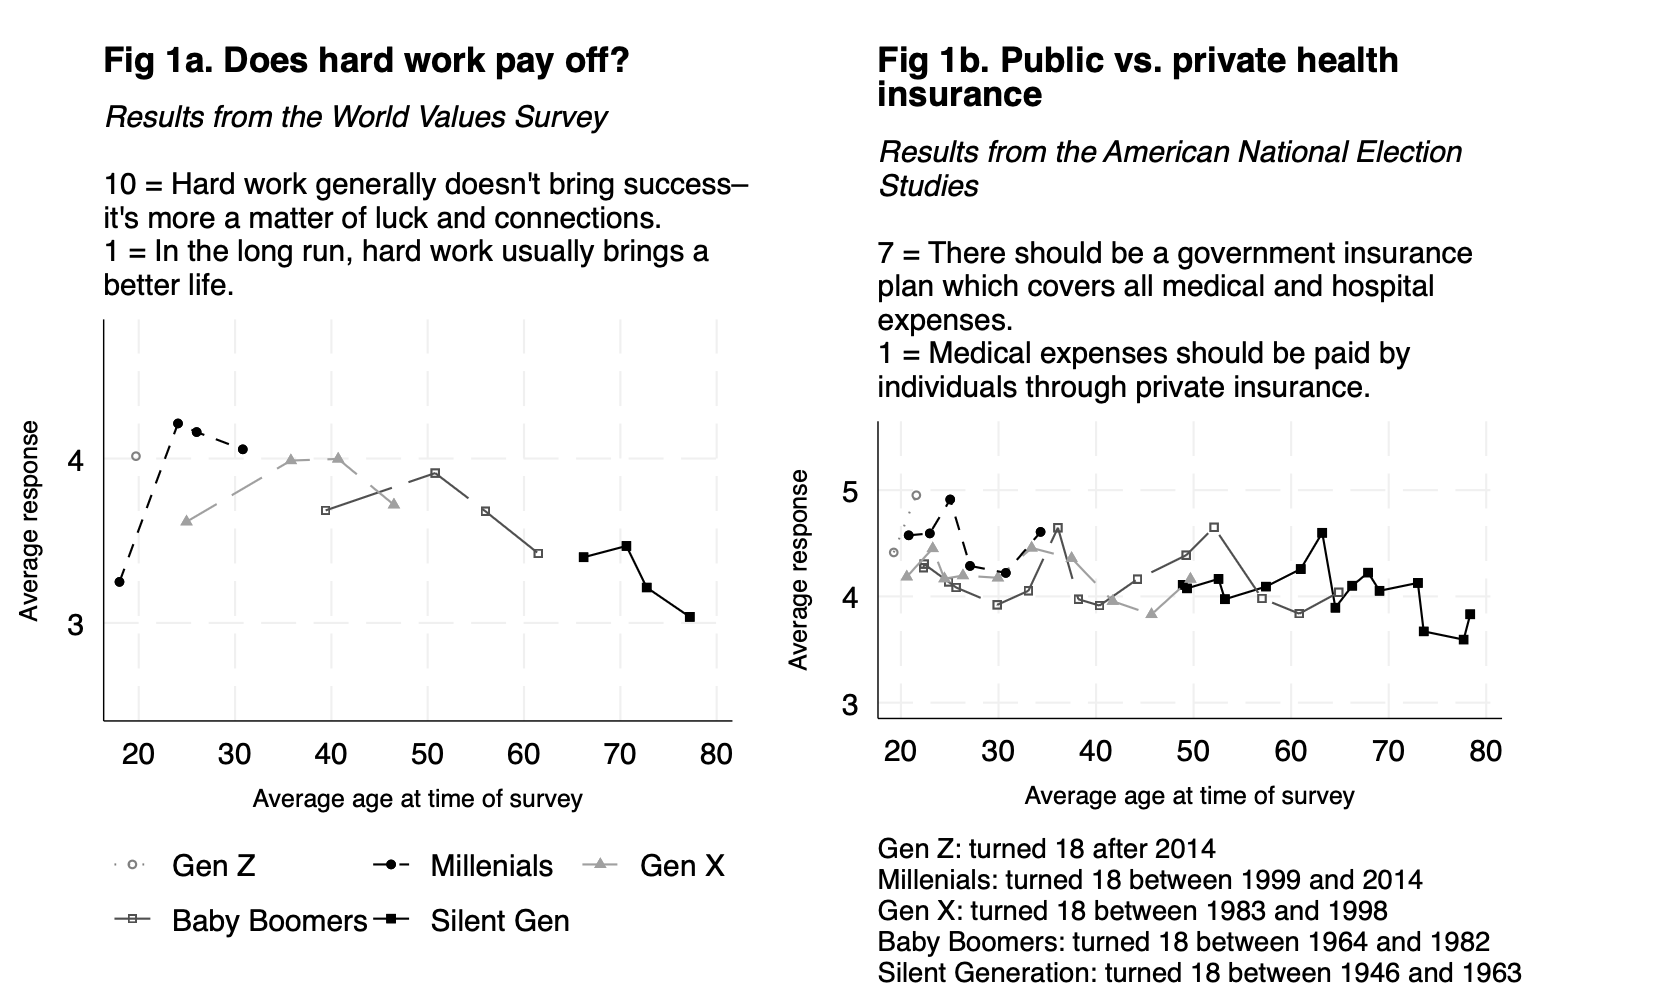
\includegraphics[width=\linewidth]{images/long_age1.png}
% \end{figure}
% \begin{figure}[H]
%     \centering
%     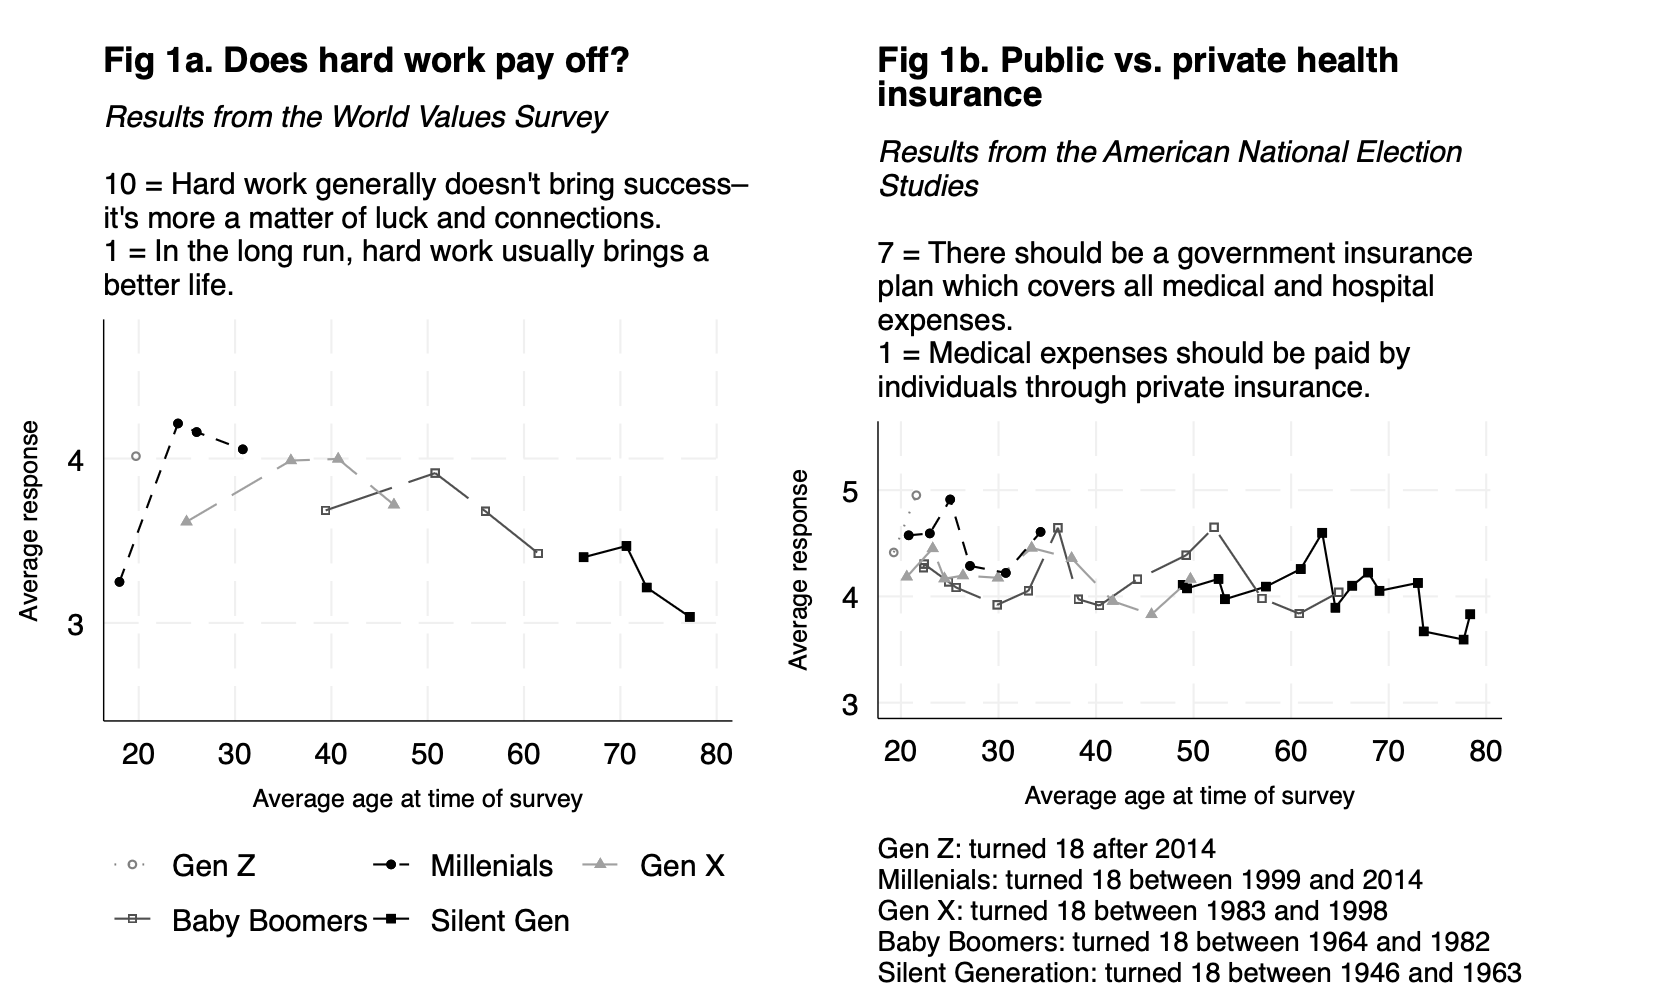
\includegraphics[width=\linewidth]{images/long_age1.png}
% \end{figure}
% \begin{figure}[H]
%     \centering
%     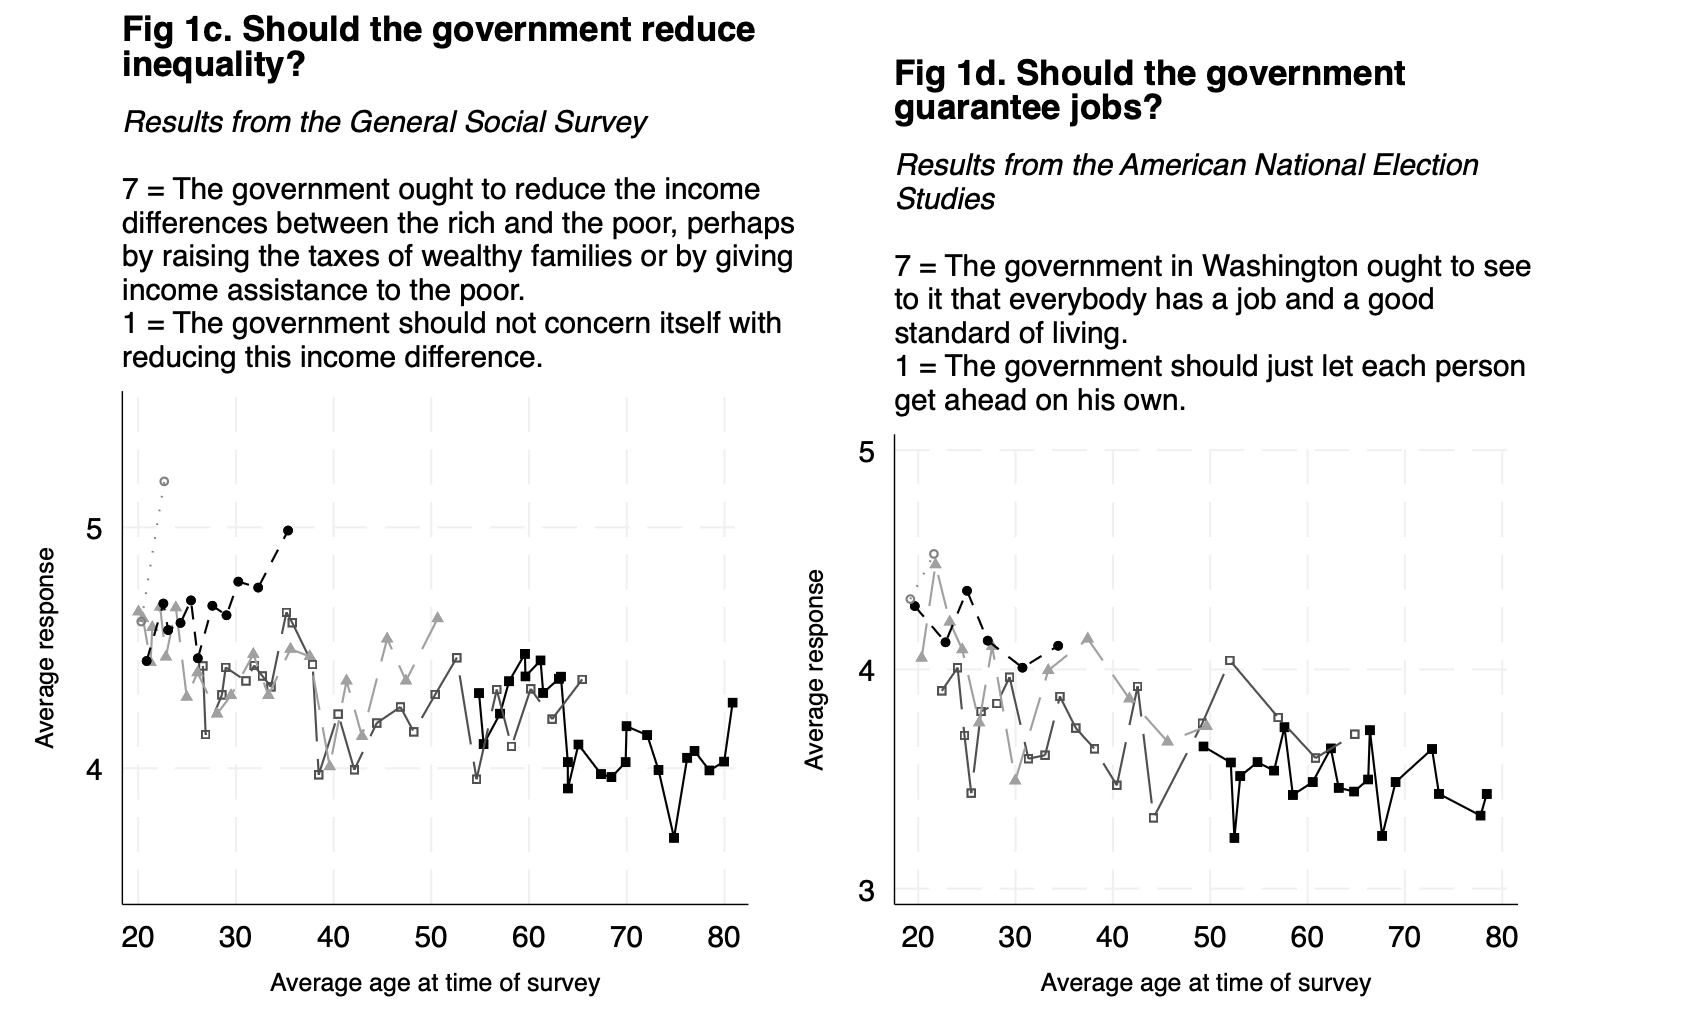
\includegraphics[width=\linewidth]{images/long_age2.png}
% \end{figure}

\newpage
\section*{Cross-sectional age gradient}

\subsection*{Prolific survey}

\begin{figure}[H]
    \centering
    \caption{Support for redistribution young vs. old}
    \begin{subfigure}{.45\textwidth}
        \centering
        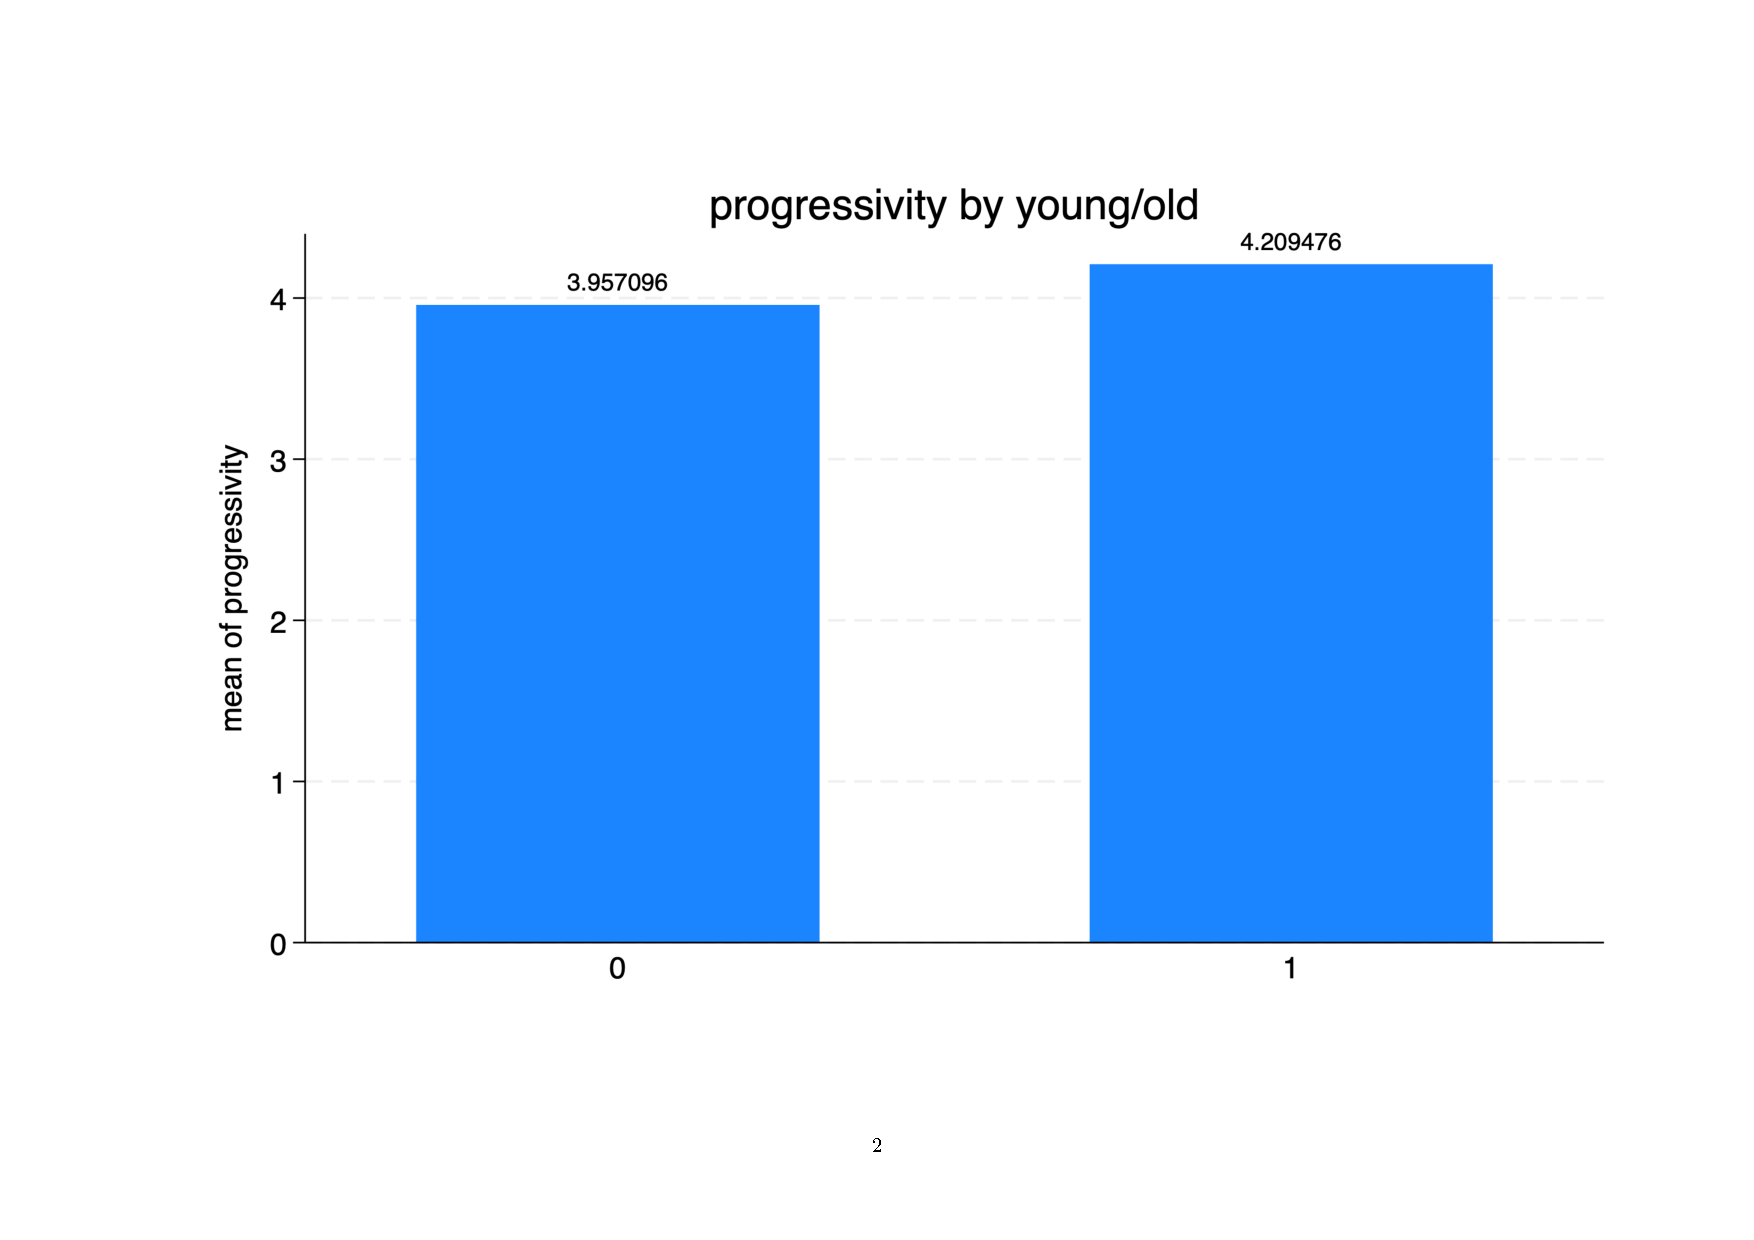
\includegraphics[width=\linewidth]{images/youngold_progressivity.pdf}
    \end{subfigure}
    \begin{subfigure}{.45\textwidth}
        \centering
        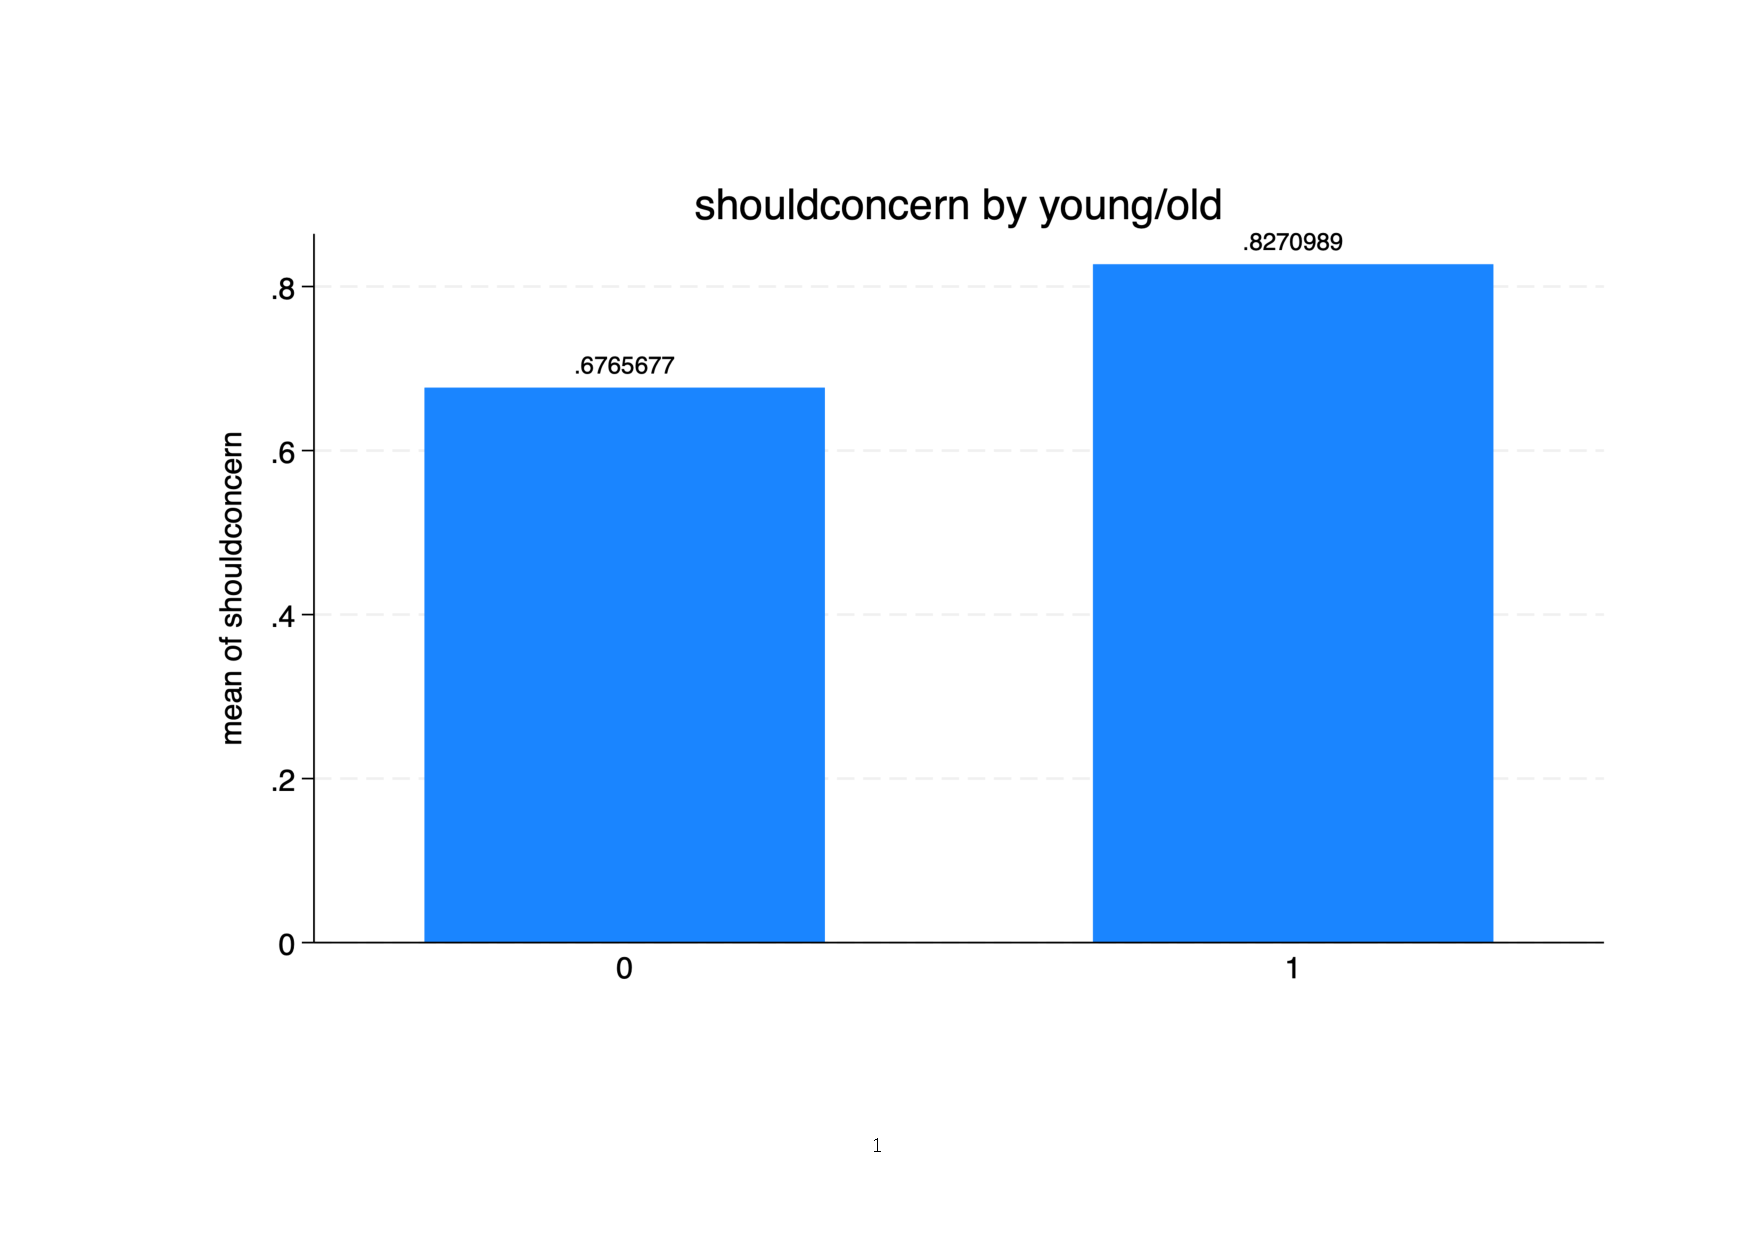
\includegraphics[width=\linewidth]{images/youngold_shouldconcern.pdf}
    \end{subfigure}
\end{figure}

\begin{figure}[H]
    \centering
    \caption{Support for redistribution by age group}
    \begin{subfigure}{.49\textwidth}
        \centering
        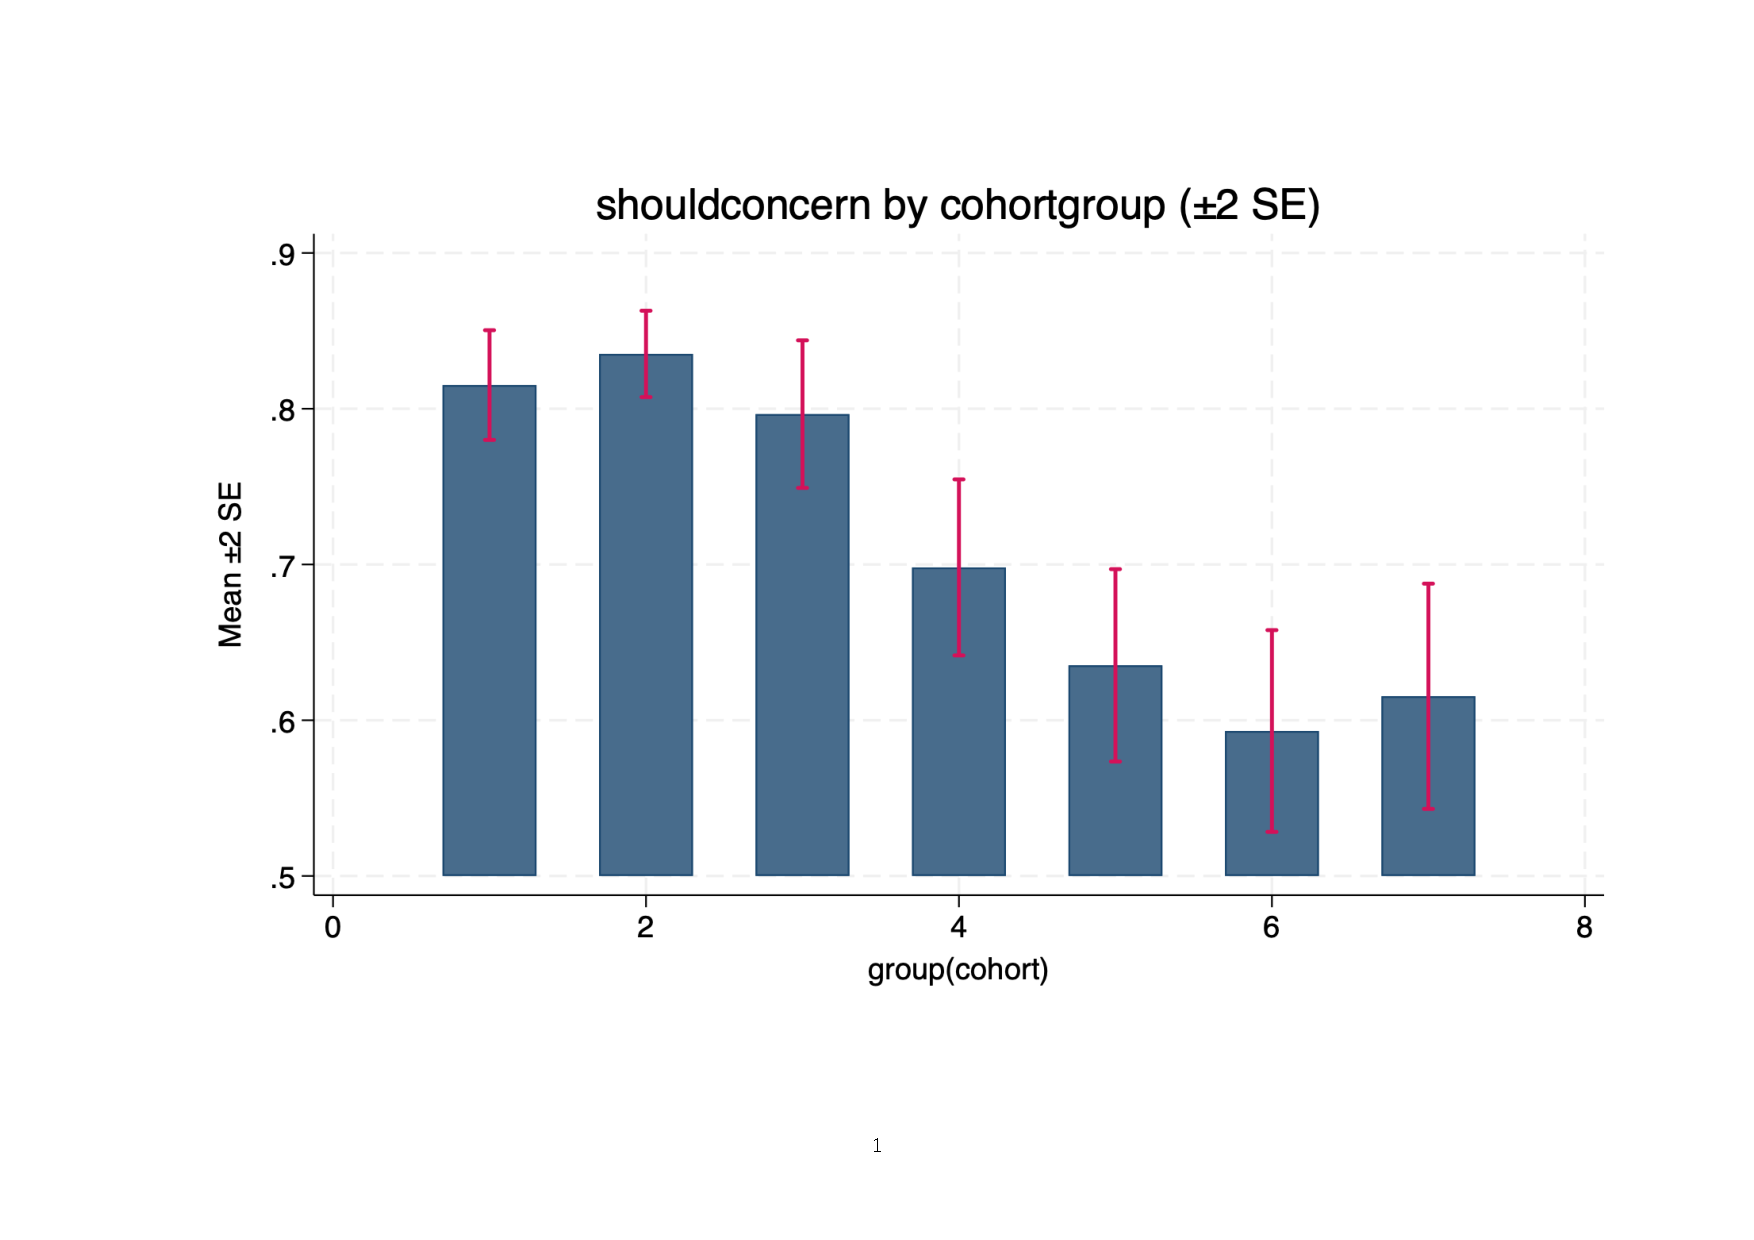
\includegraphics[width=\linewidth]{images/cohort_shouldconcern.pdf}
    \end{subfigure}
    \begin{subfigure}{.49\textwidth}
        \centering
        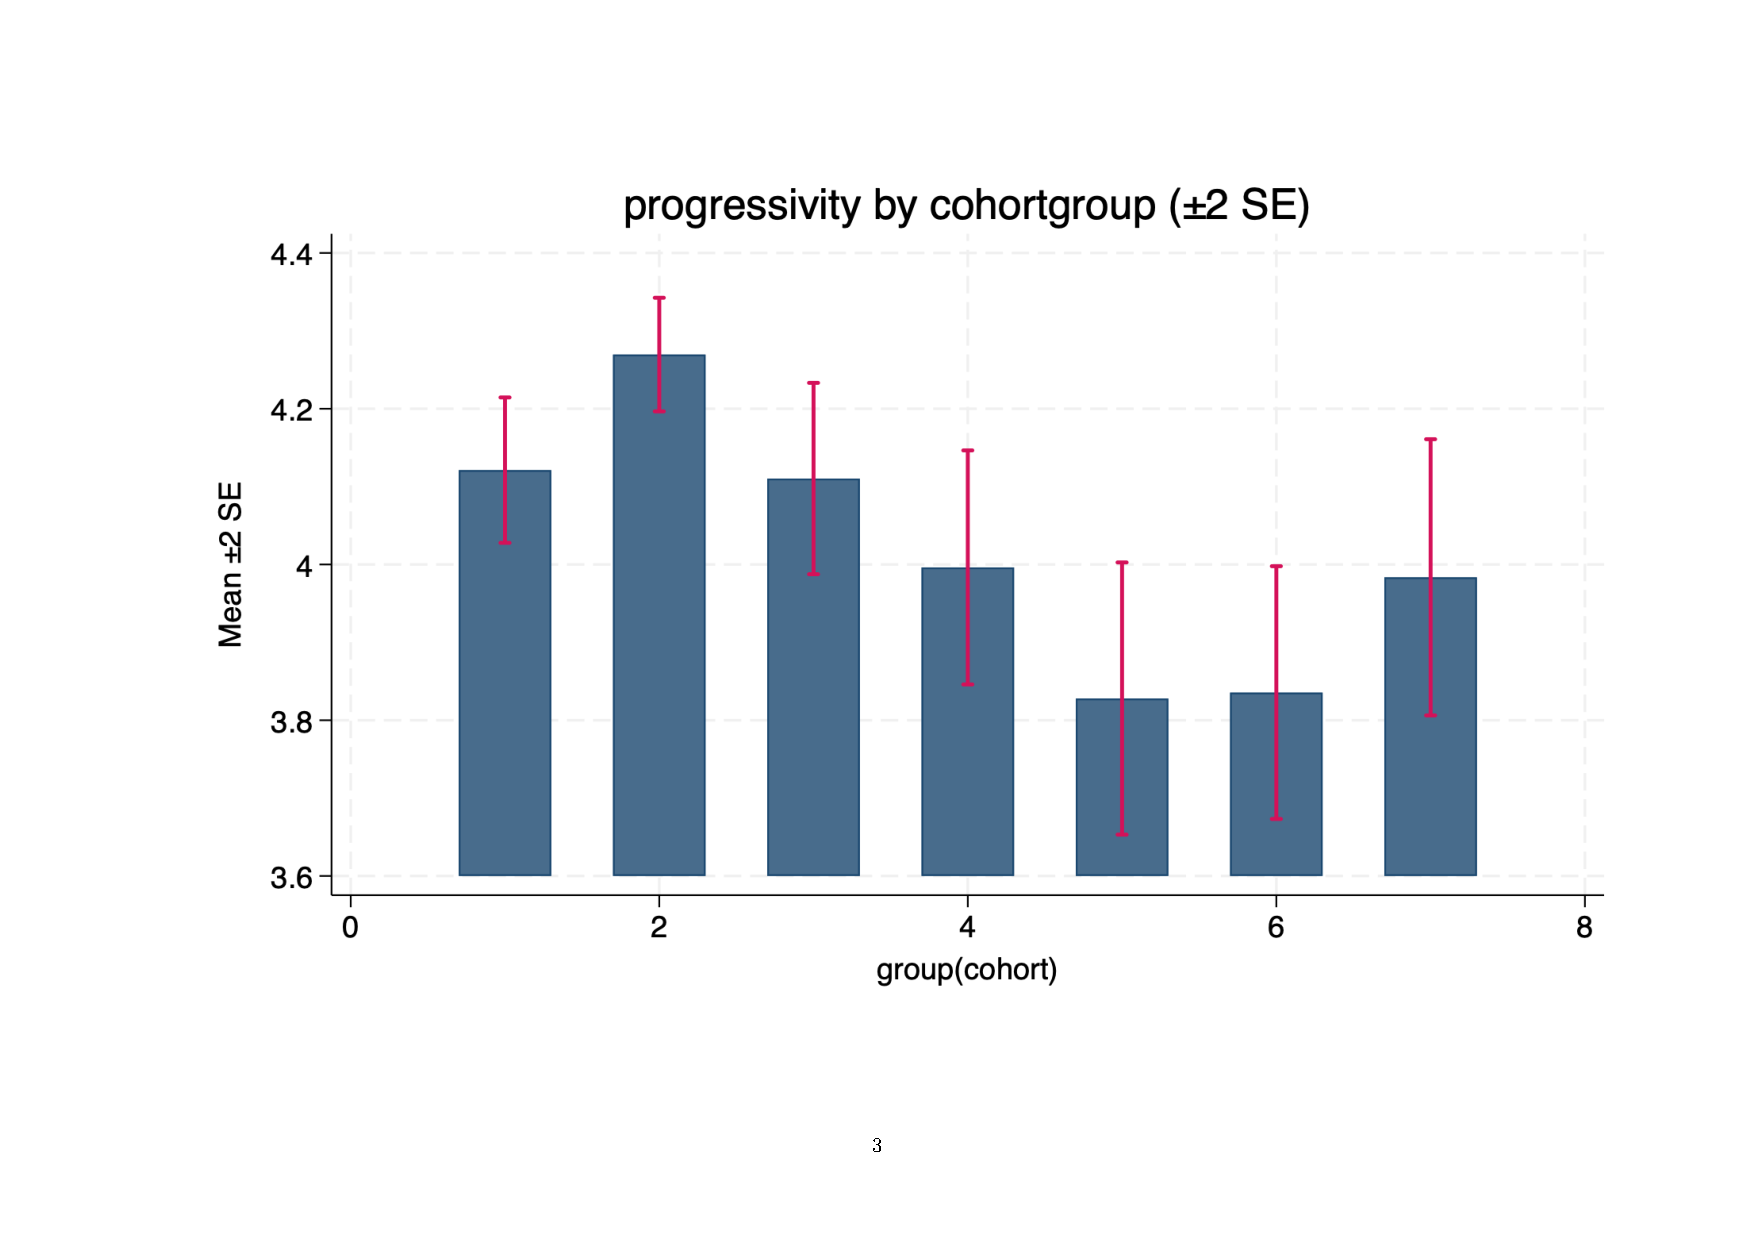
\includegraphics[width=\linewidth]{images/cohort_progressivity.pdf}
    \end{subfigure}
\end{figure}

\begin{figure}[H]
    \centering
    \caption{Mobility and zero-sum by age group}
    \begin{subfigure}{.49\textwidth}
        \centering
        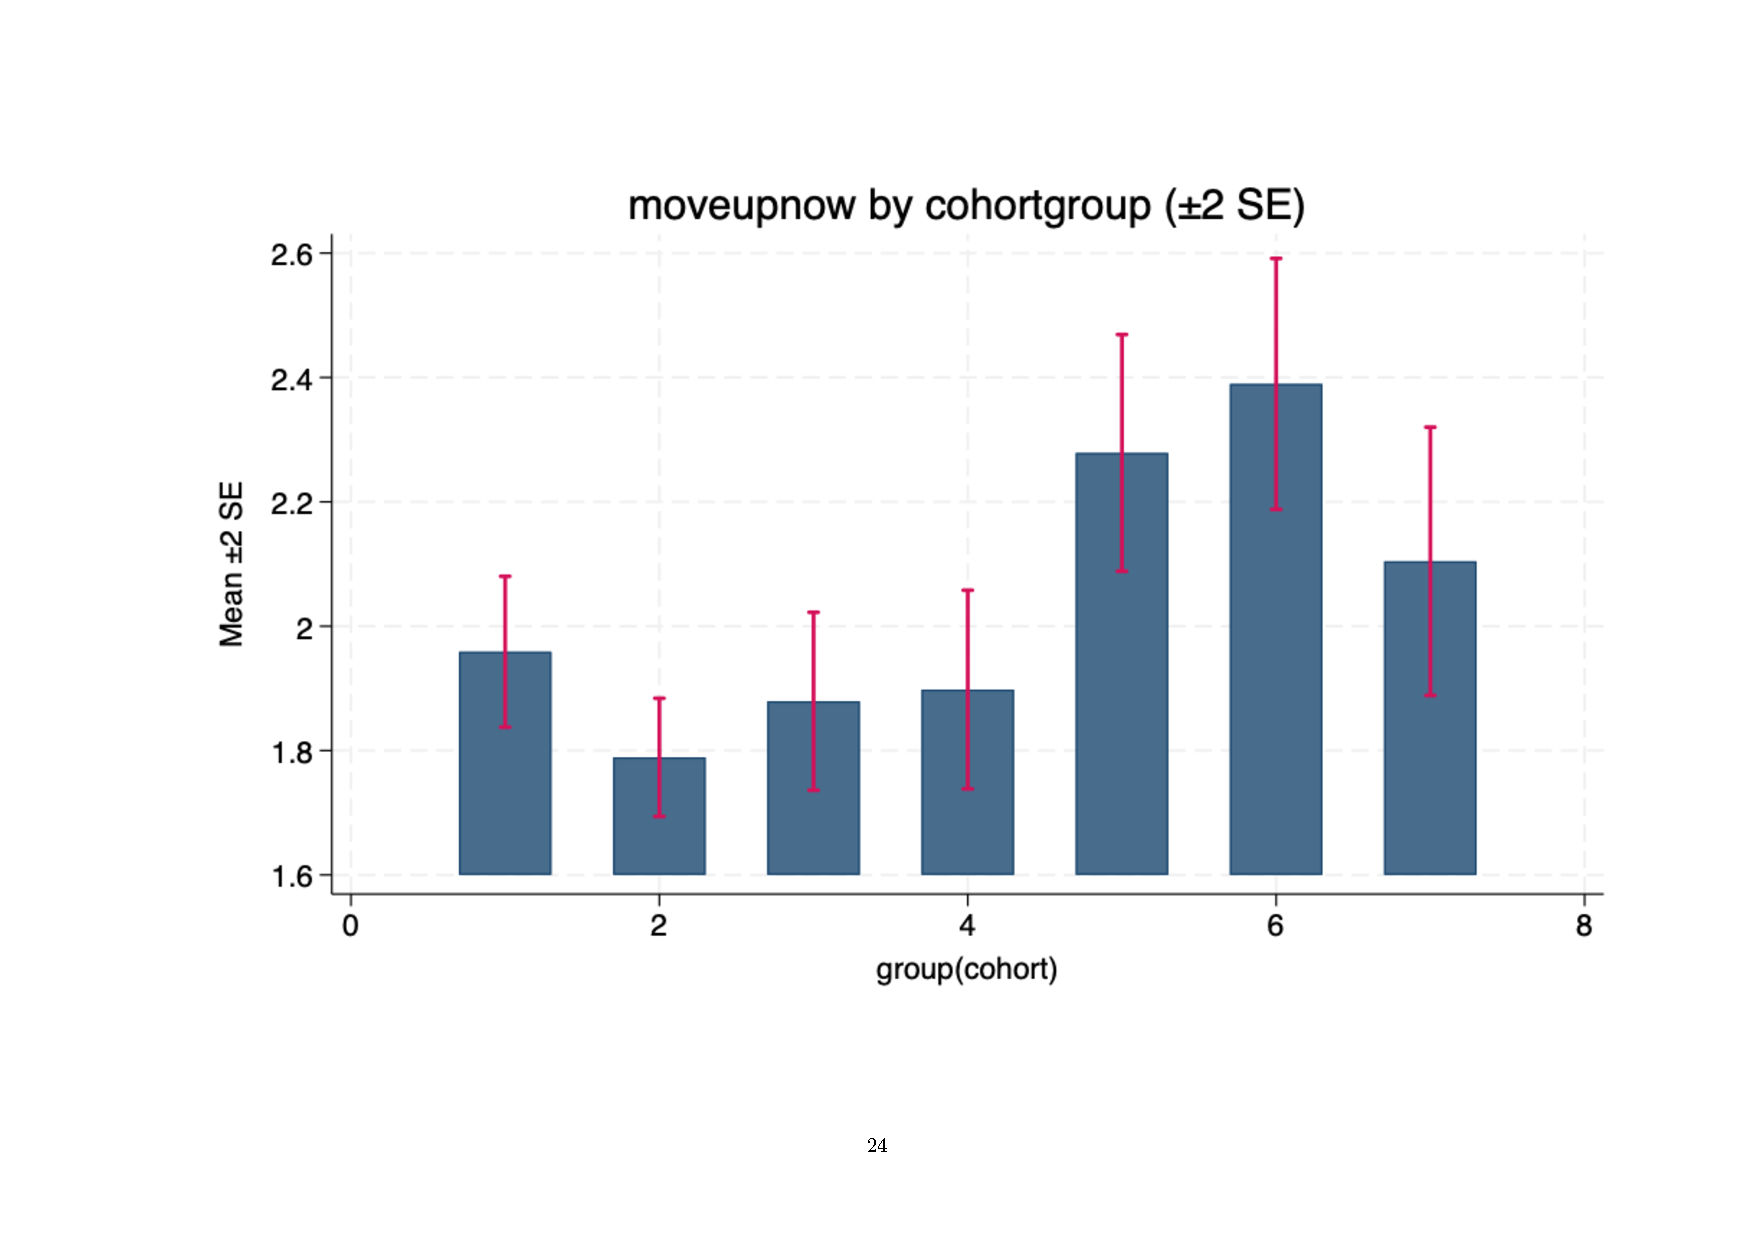
\includegraphics[width=\linewidth]{images/cohort_moveupnow.pdf}
    \end{subfigure}
    \begin{subfigure}{.49\textwidth}
        \centering
        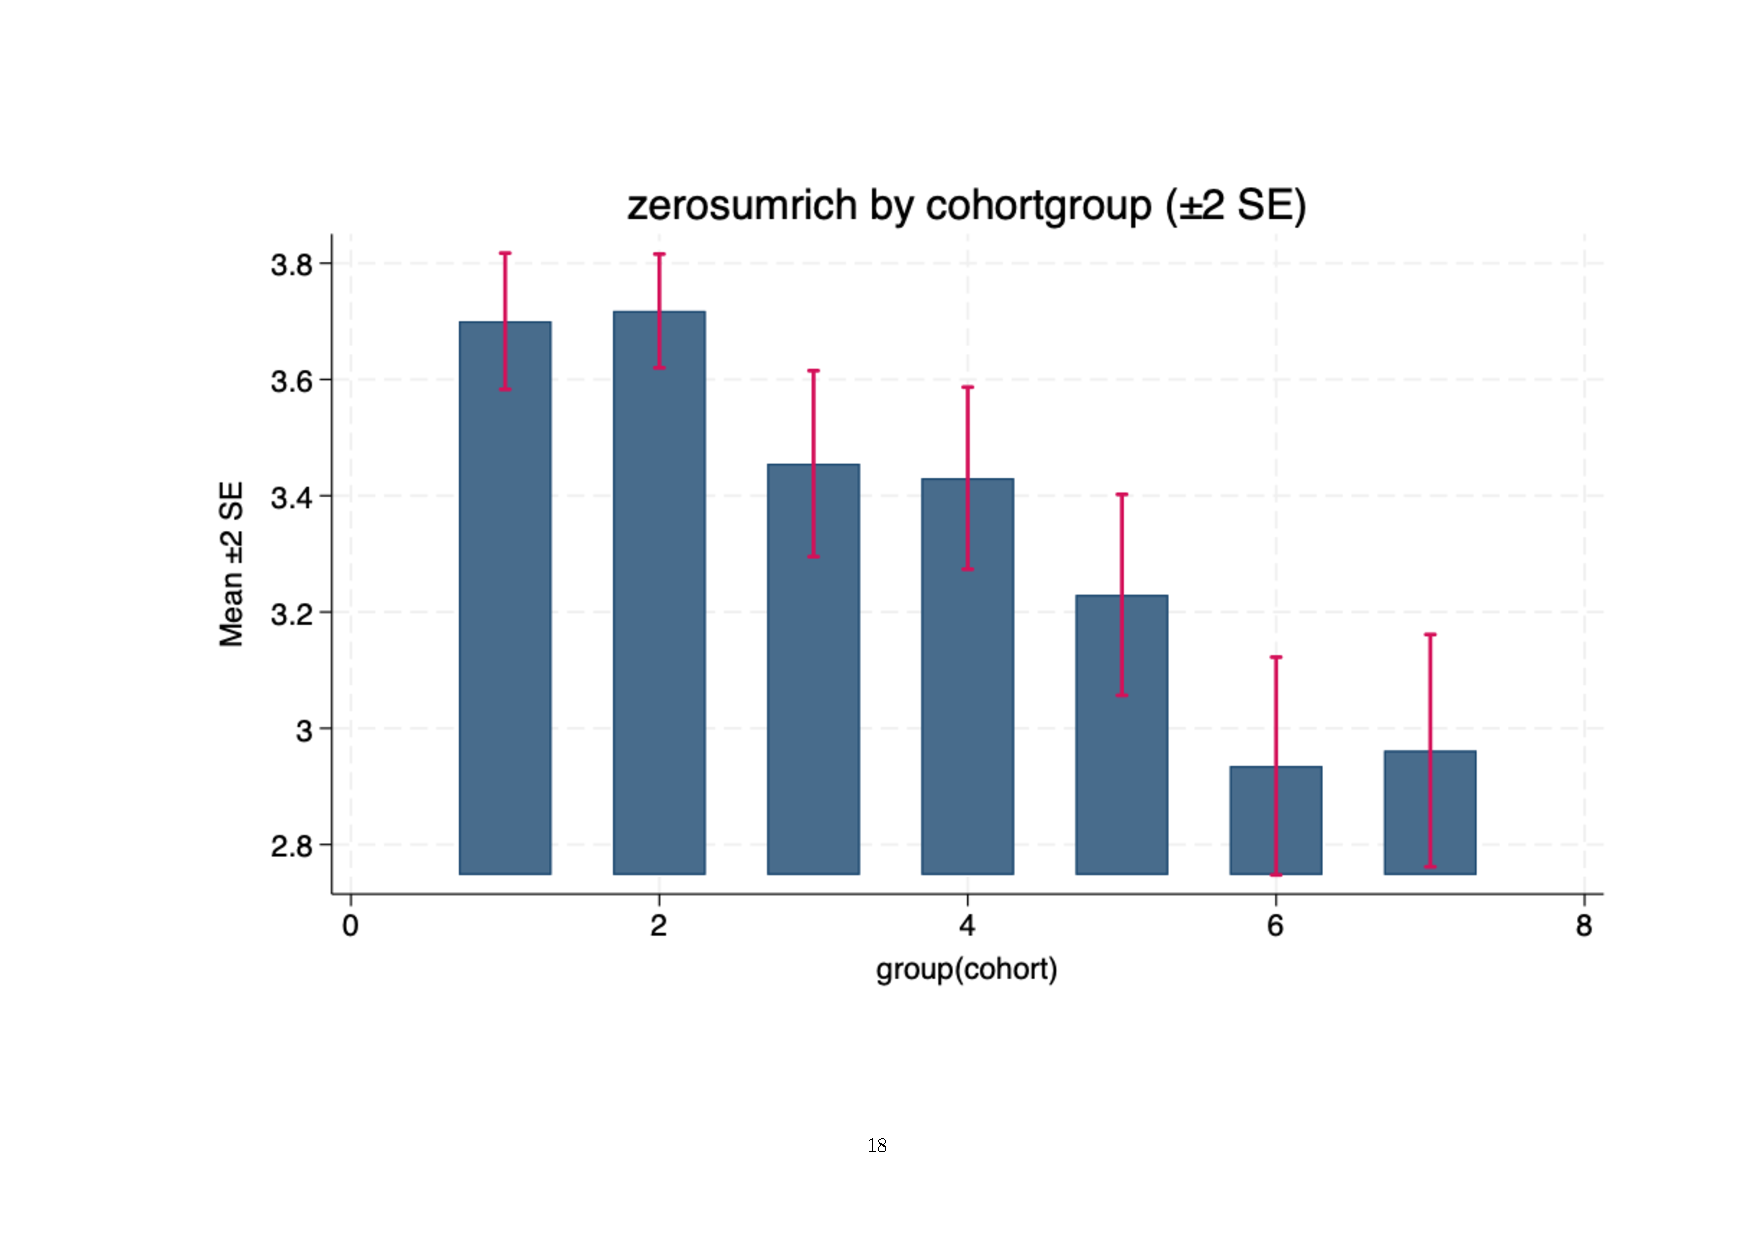
\includegraphics[width=\linewidth]{images/cohort_zerosumrich.pdf}
    \end{subfigure}
\end{figure}

\begin{figure}[H]
    \centering
    \caption{Generosity/communalism and time-discounting/marginal utility by age group}
    \begin{subfigure}{.49\textwidth}
        \centering
        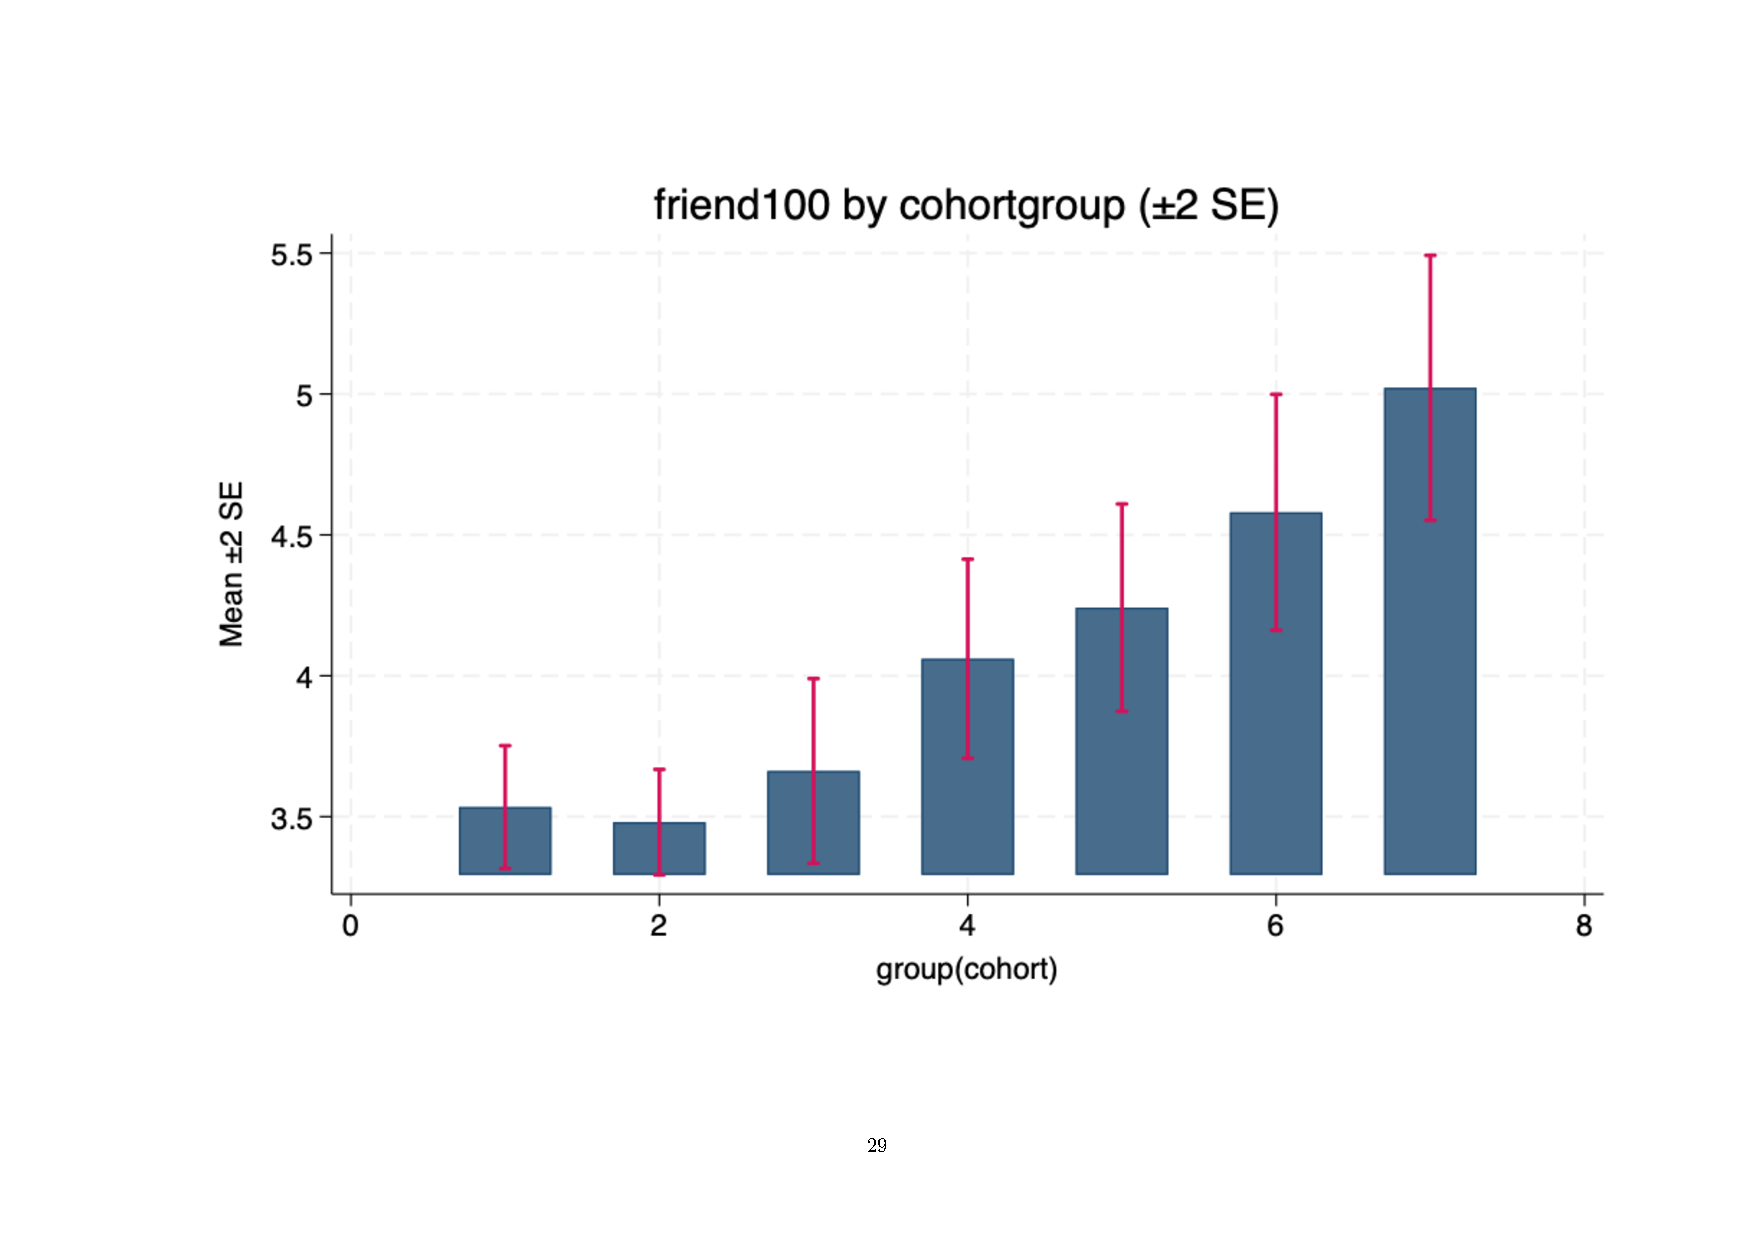
\includegraphics[width=\linewidth]{images/cohort_friend100.pdf}
    \end{subfigure}
    \begin{subfigure}{.49\textwidth}
        \centering
        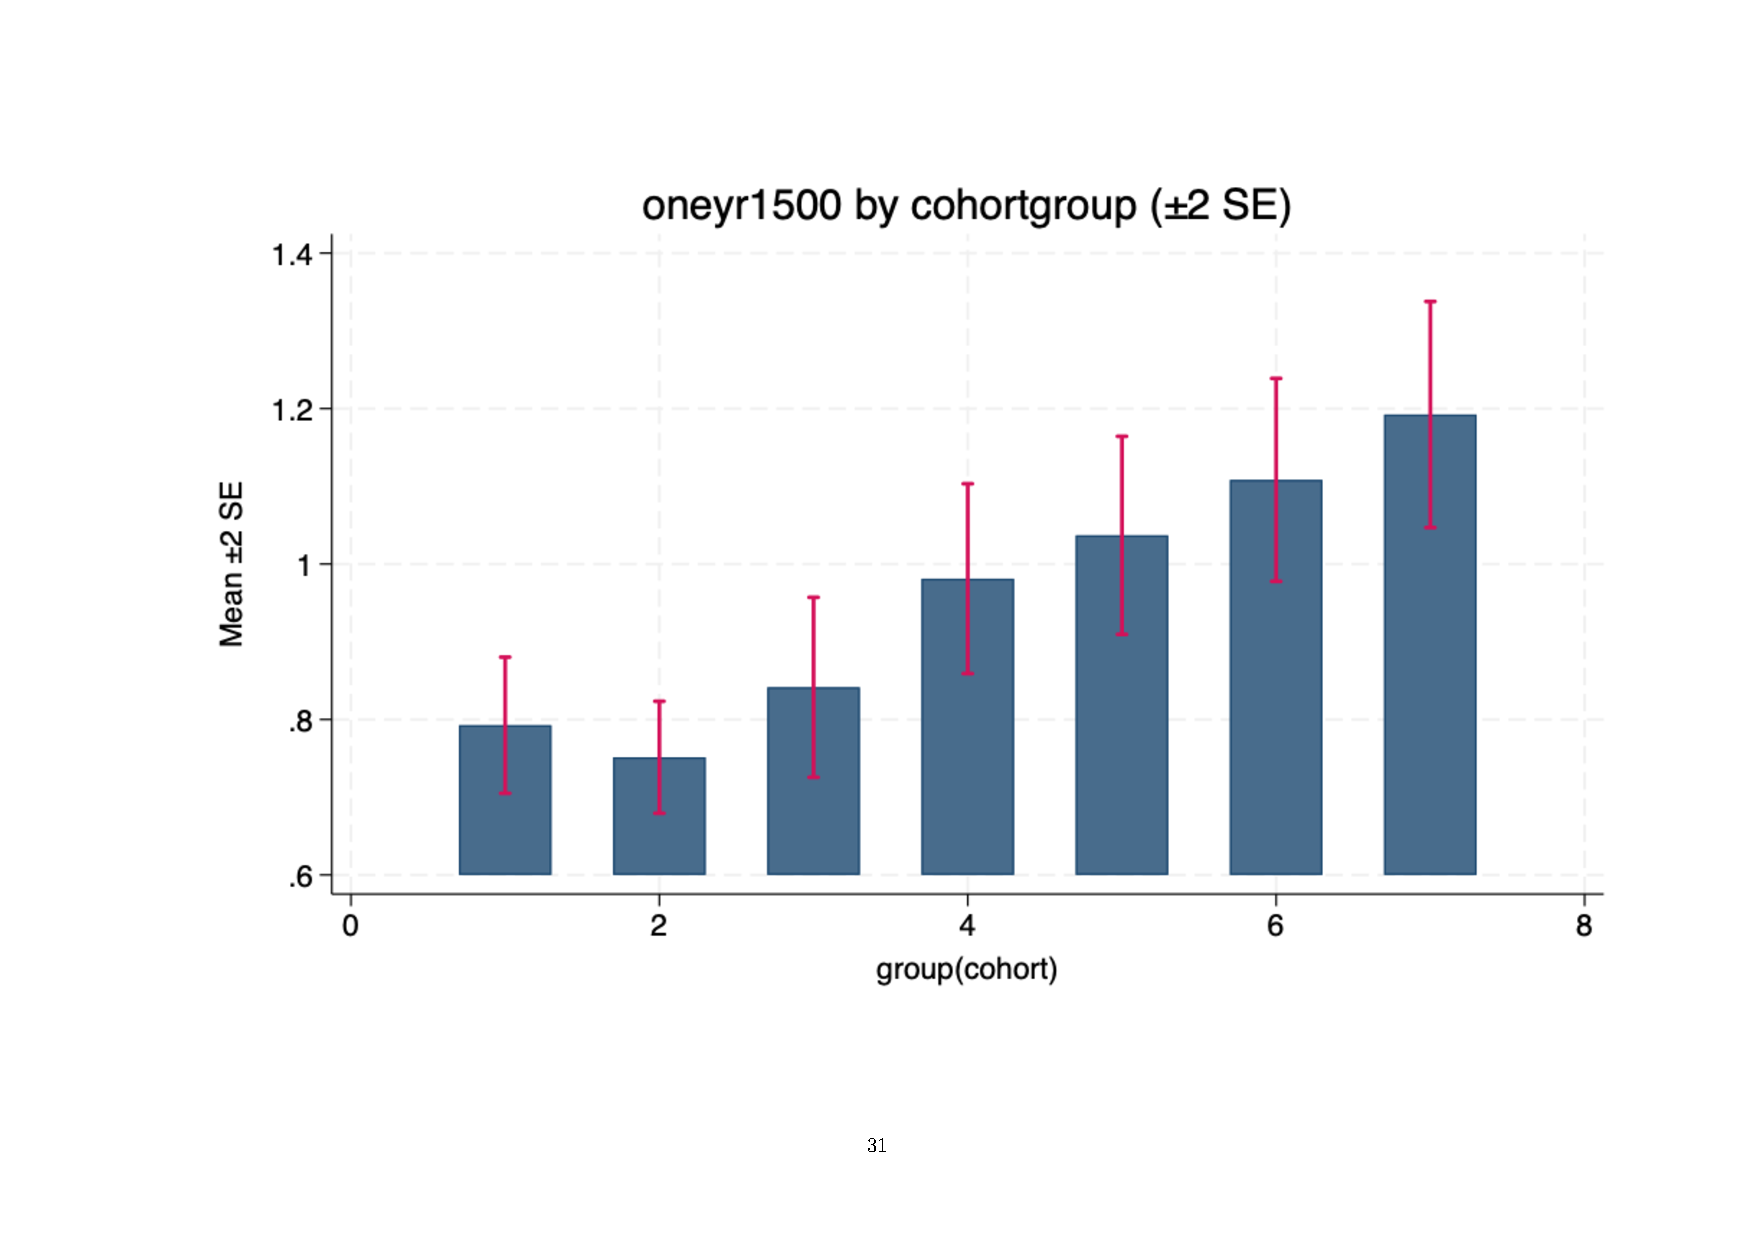
\includegraphics[width=\linewidth]{images/cohort_oneyr1500.pdf}
    \end{subfigure}
\end{figure}

\begin{figure}[H]
    \centering
    \caption{Financial concerns by age group}
    \begin{subfigure}{.49\textwidth}
        \centering
        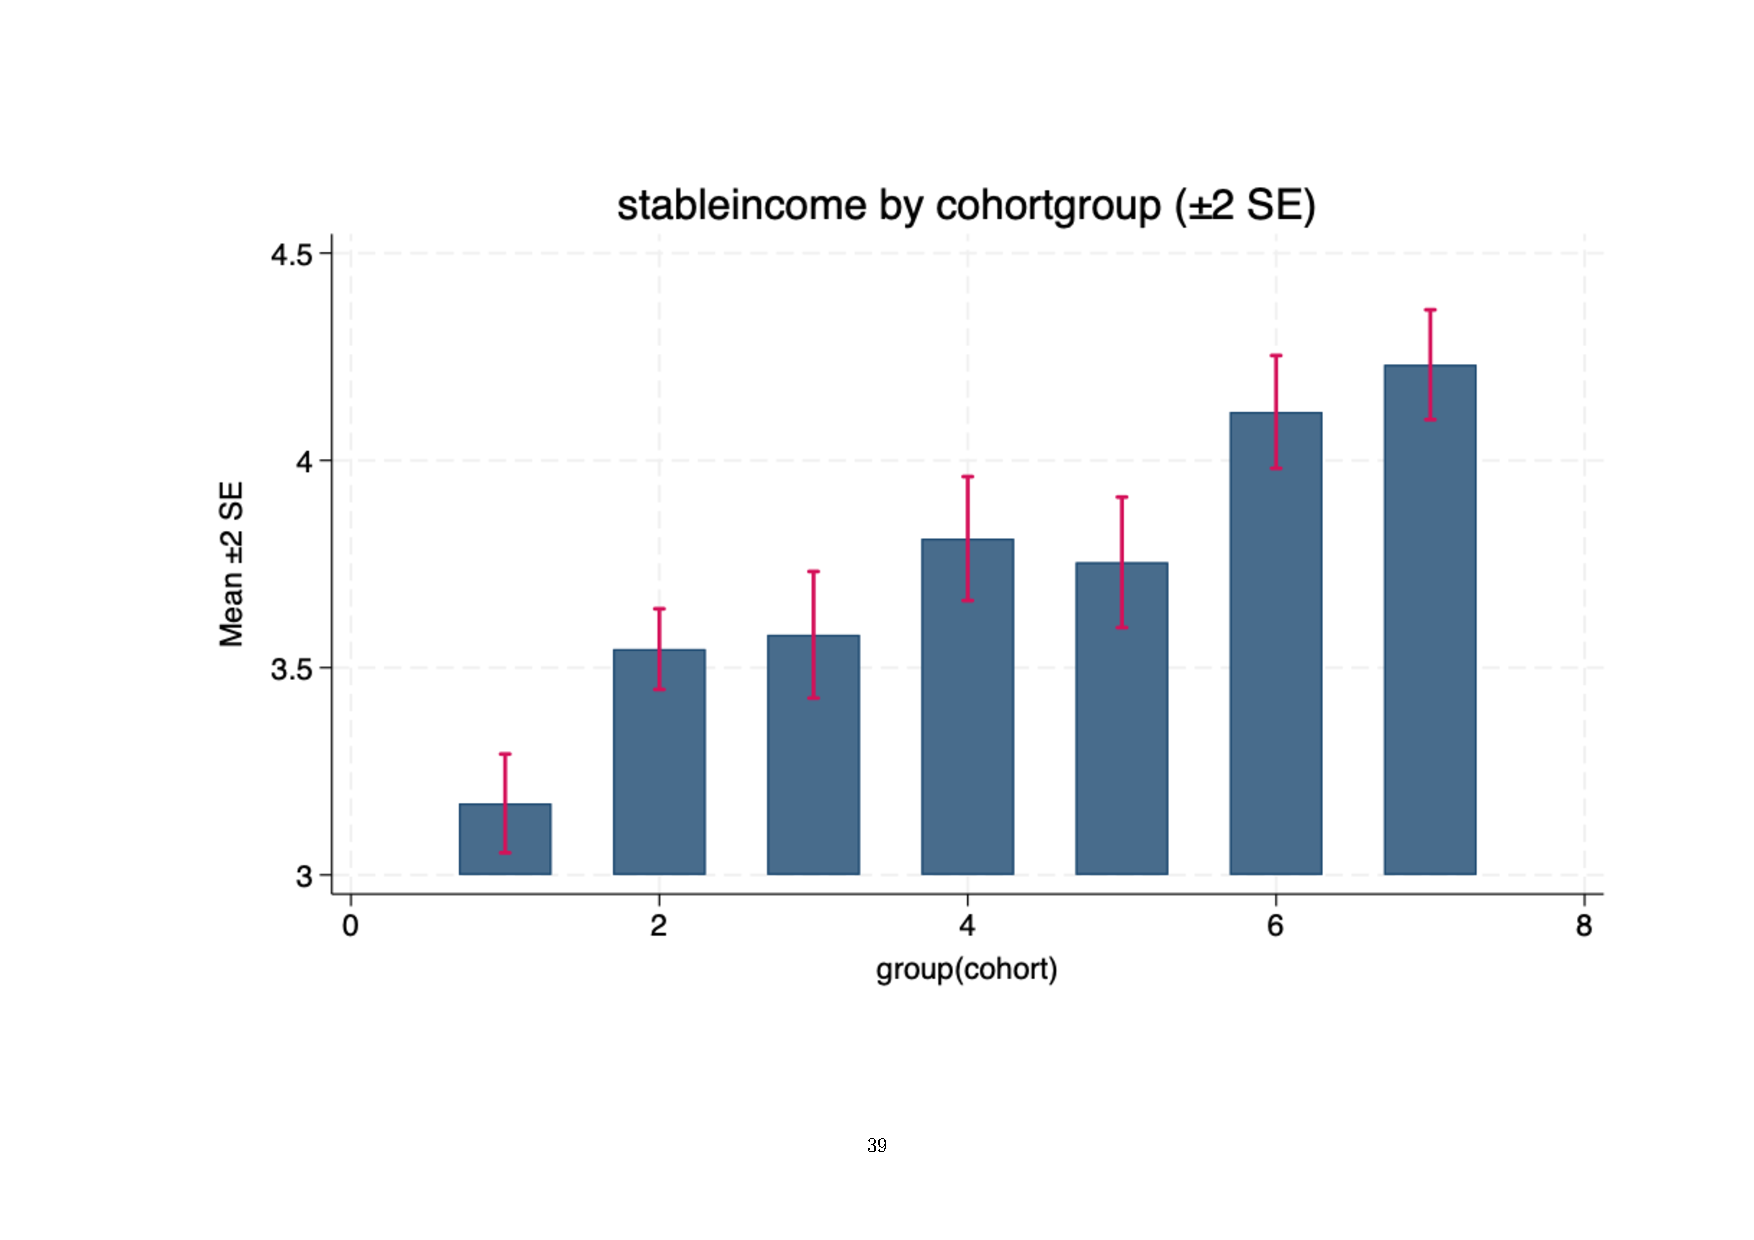
\includegraphics[width=\linewidth]{images/cohort_stableincome.pdf}
    \end{subfigure}
    \begin{subfigure}{.49\textwidth}
        \centering
        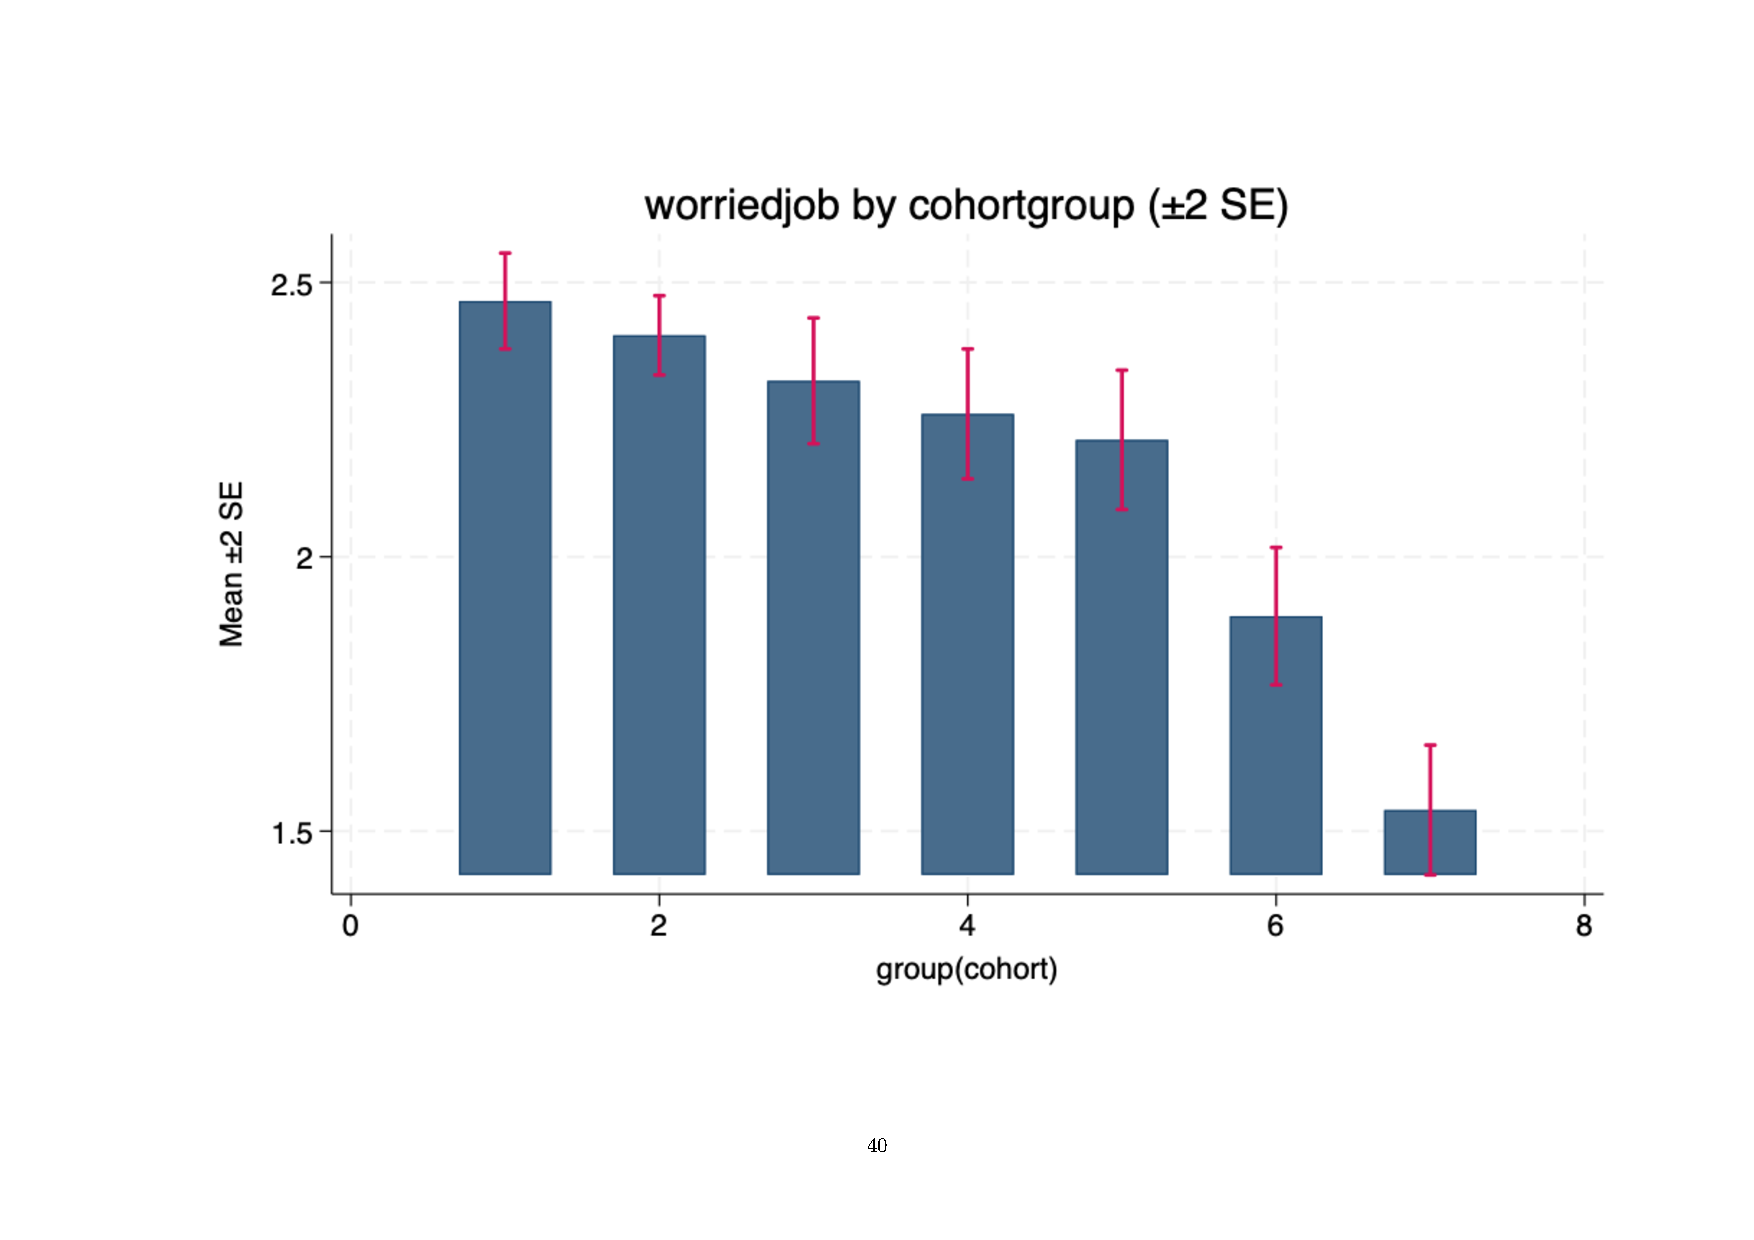
\includegraphics[width=\linewidth]{images/cohort_worriedjob.pdf}
    \end{subfigure}
\end{figure}
\begin{figure}[H]
    \centering
    \caption{Safety net and housing risk by age group}
    \begin{subfigure}{.49\textwidth}
        \centering
        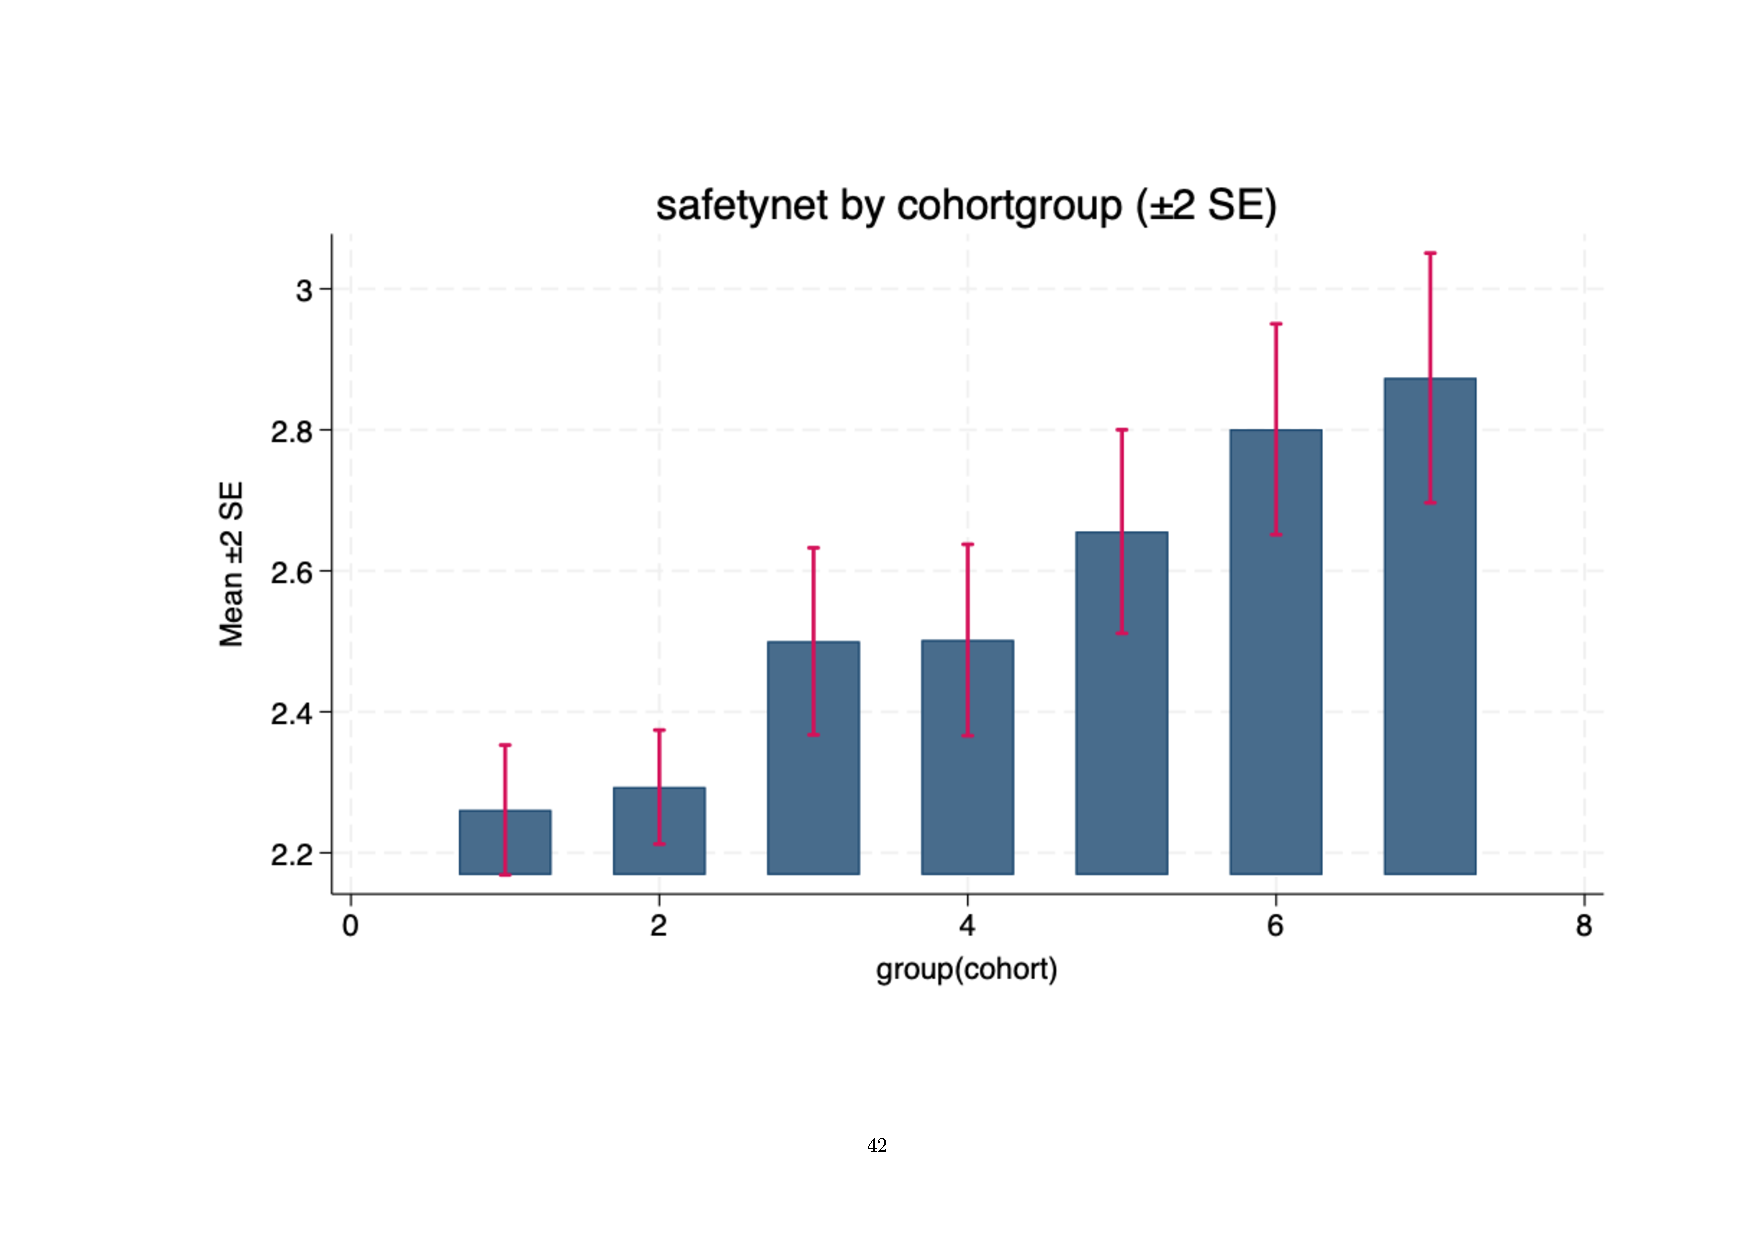
\includegraphics[width=\linewidth]{images/cohort_safetynet.pdf}
    \end{subfigure}
    \begin{subfigure}{.49\textwidth}
        \centering
        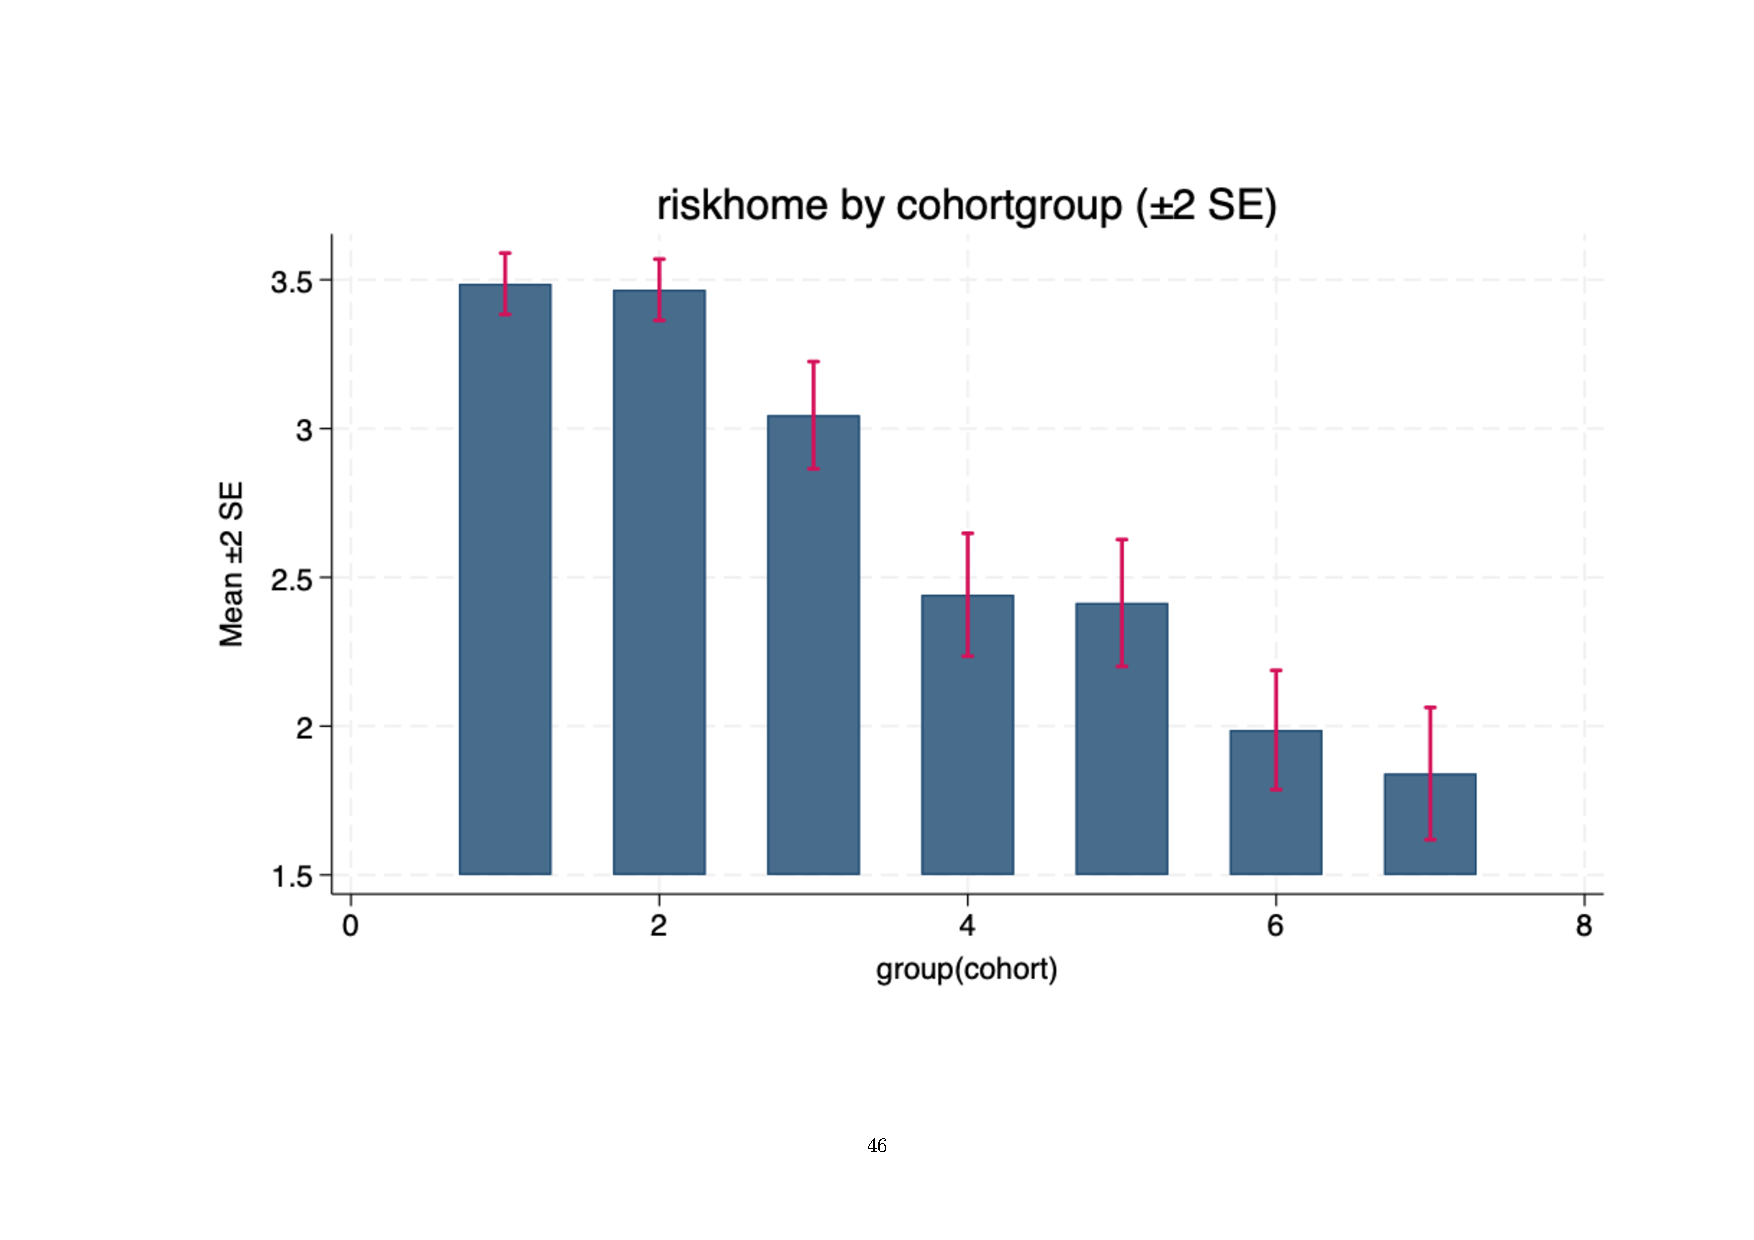
\includegraphics[width=\linewidth]{images/cohort_riskhome.pdf}
    \end{subfigure}
\end{figure}

\subsection*{Stantcheva (2005)}

\begin{figure}[H]
    \centering
    \caption{Redistributive preferences}
    \begin{subfigure}{.49\textwidth}
        \centering
        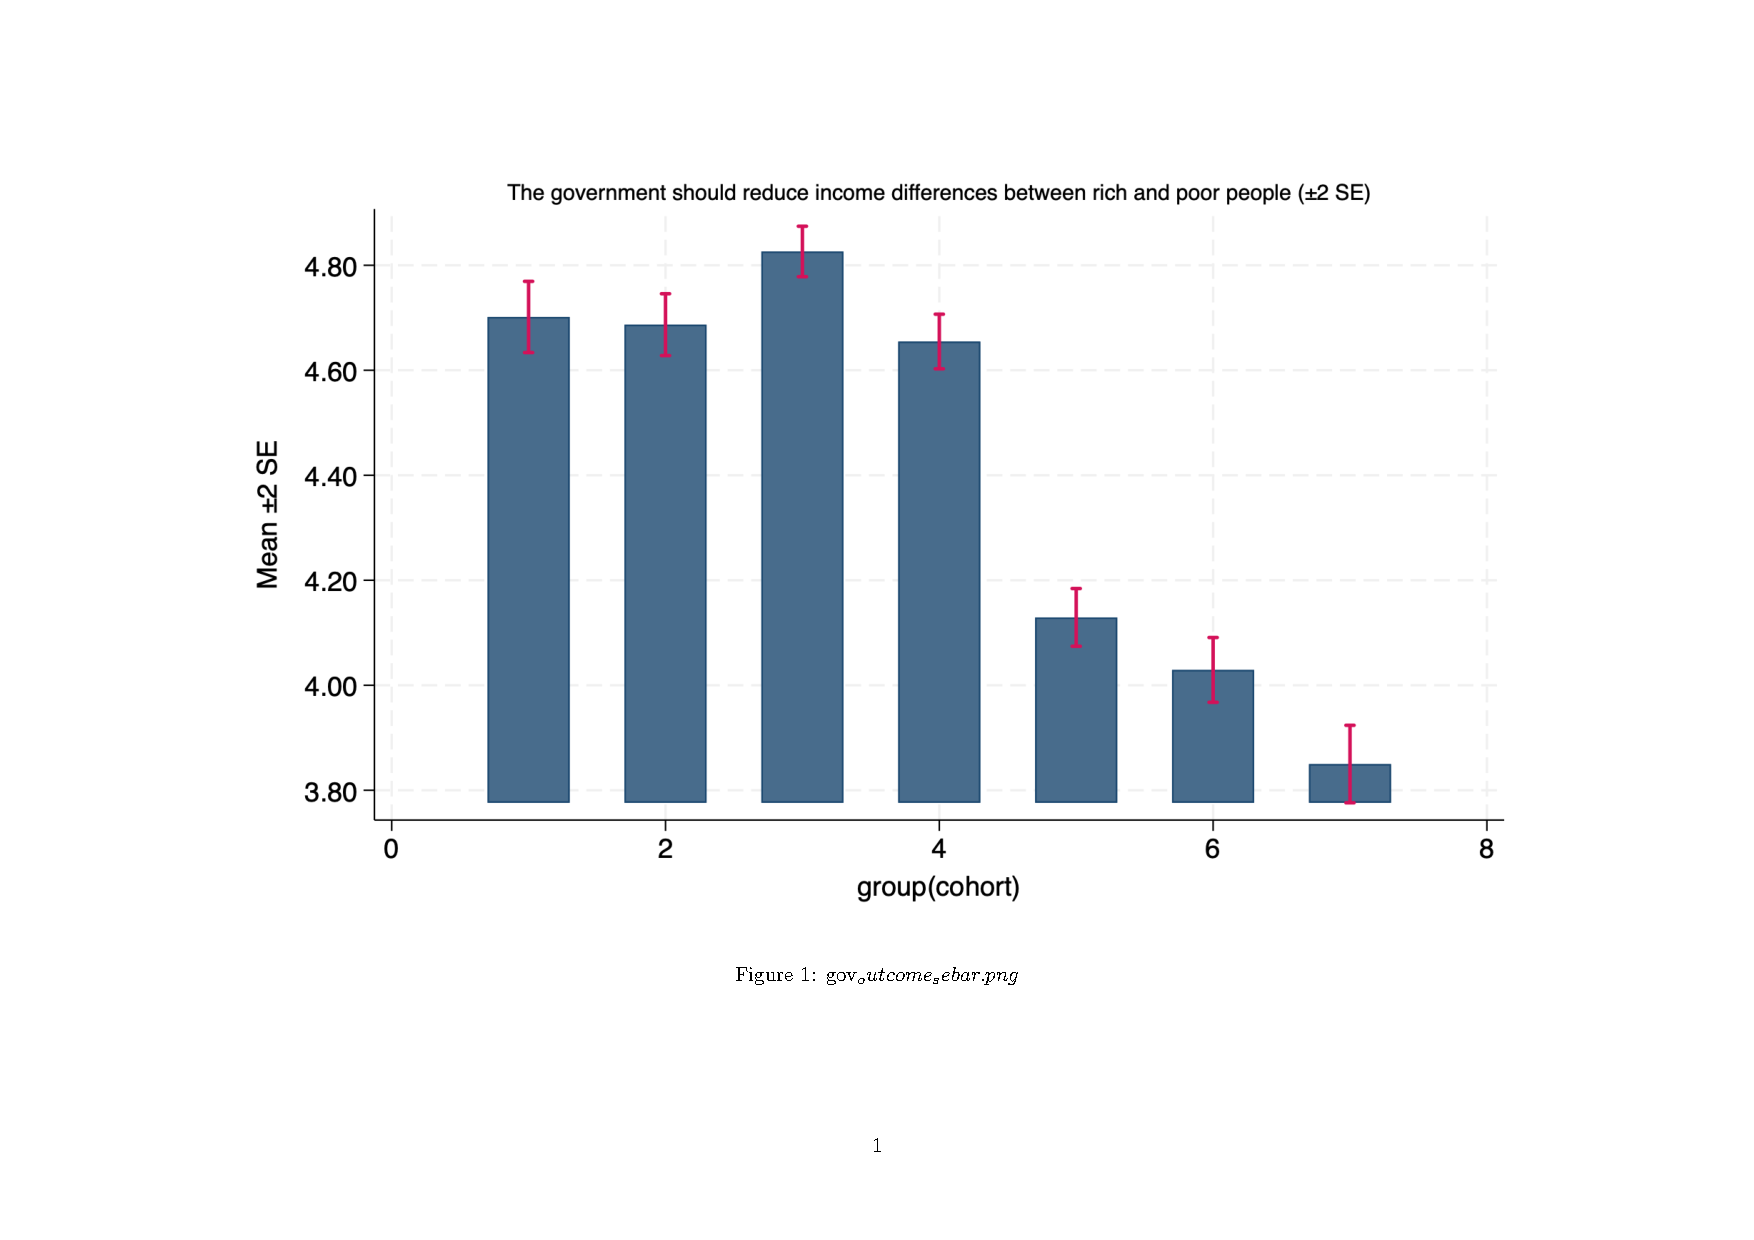
\includegraphics[width=\linewidth]{images/stantcheva2005_reducediffs.pdf}
    \end{subfigure}
\end{figure}
\begin{figure}[H]
    \centering
    \caption{Zero-sum wealth}
    \begin{subfigure}{.49\textwidth}
        \centering
        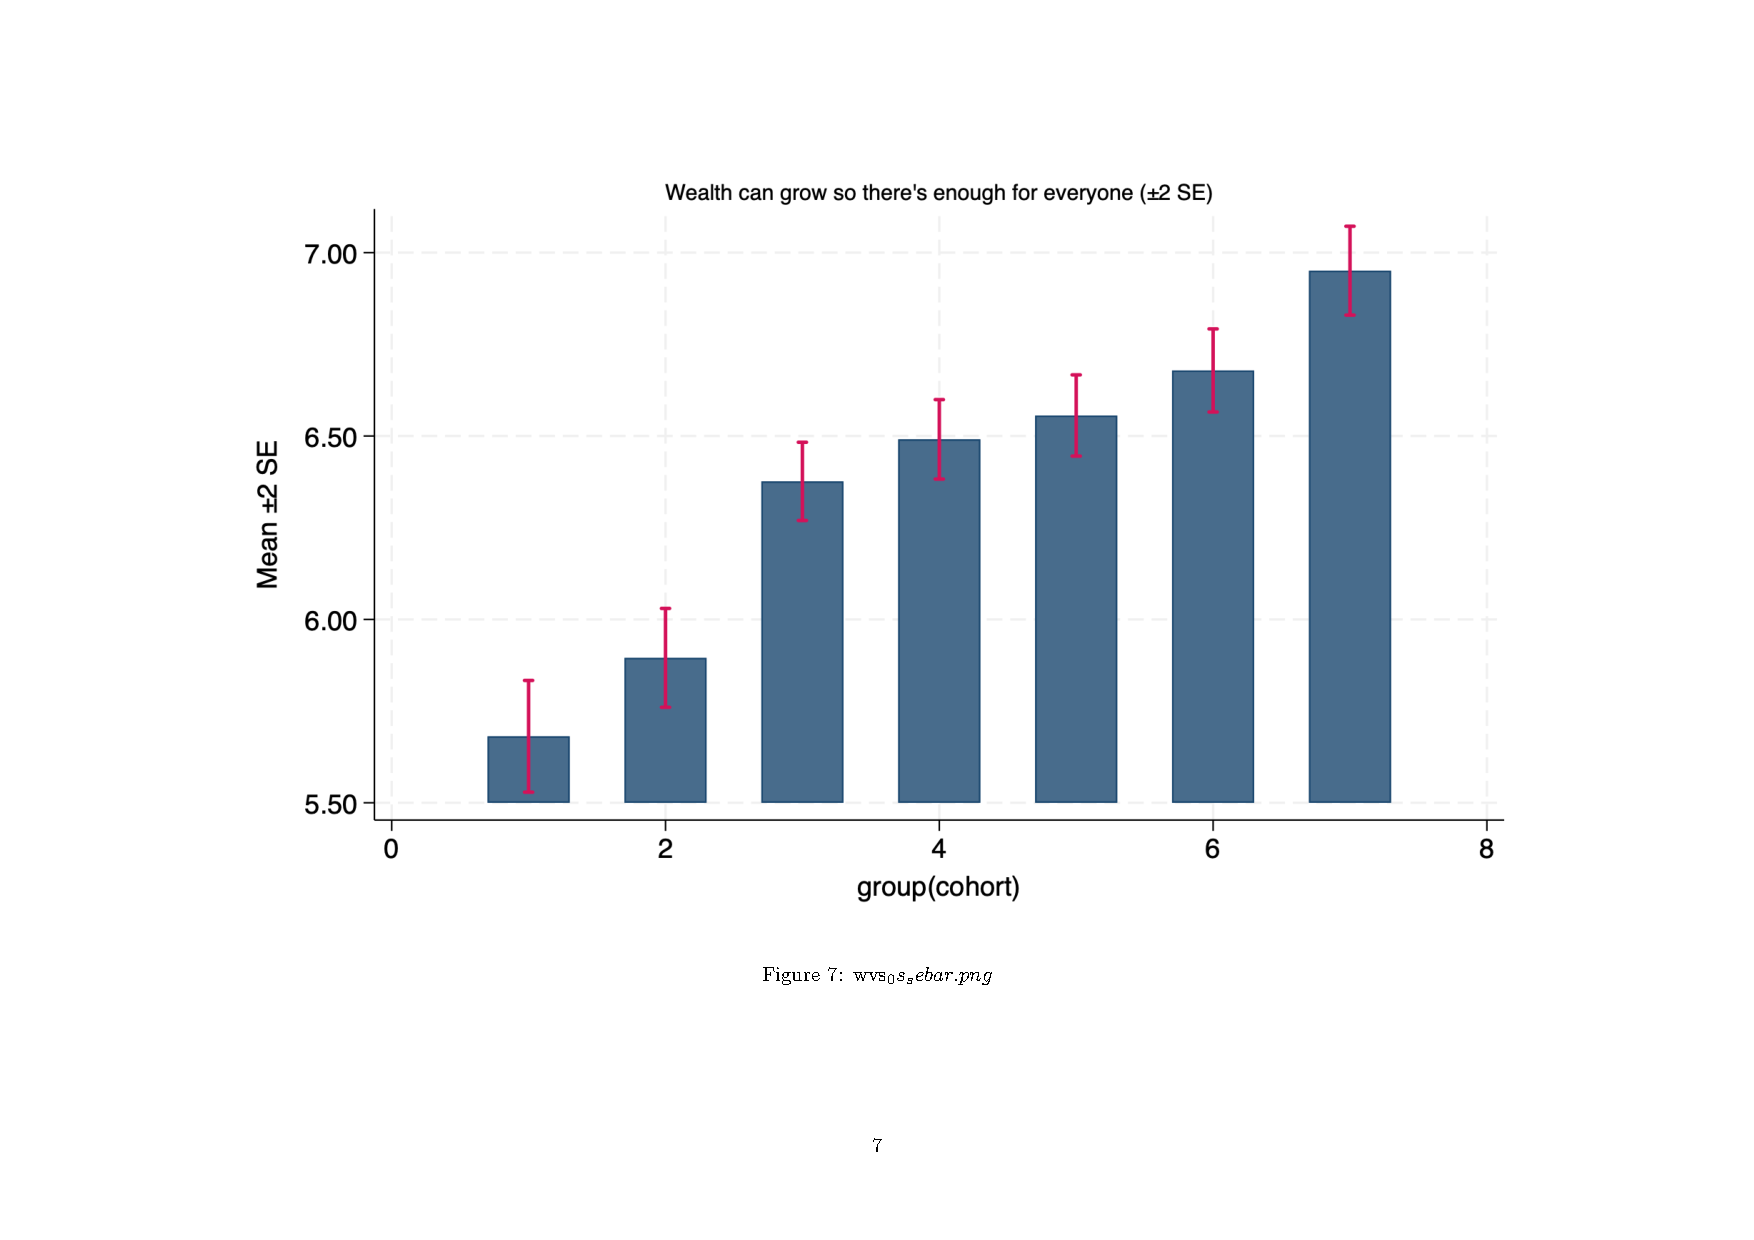
\includegraphics[width=\linewidth]{images/stantcheva2005_wealthcangrow.pdf}
    \end{subfigure}
    \begin{subfigure}{.49\textwidth}
        \centering
        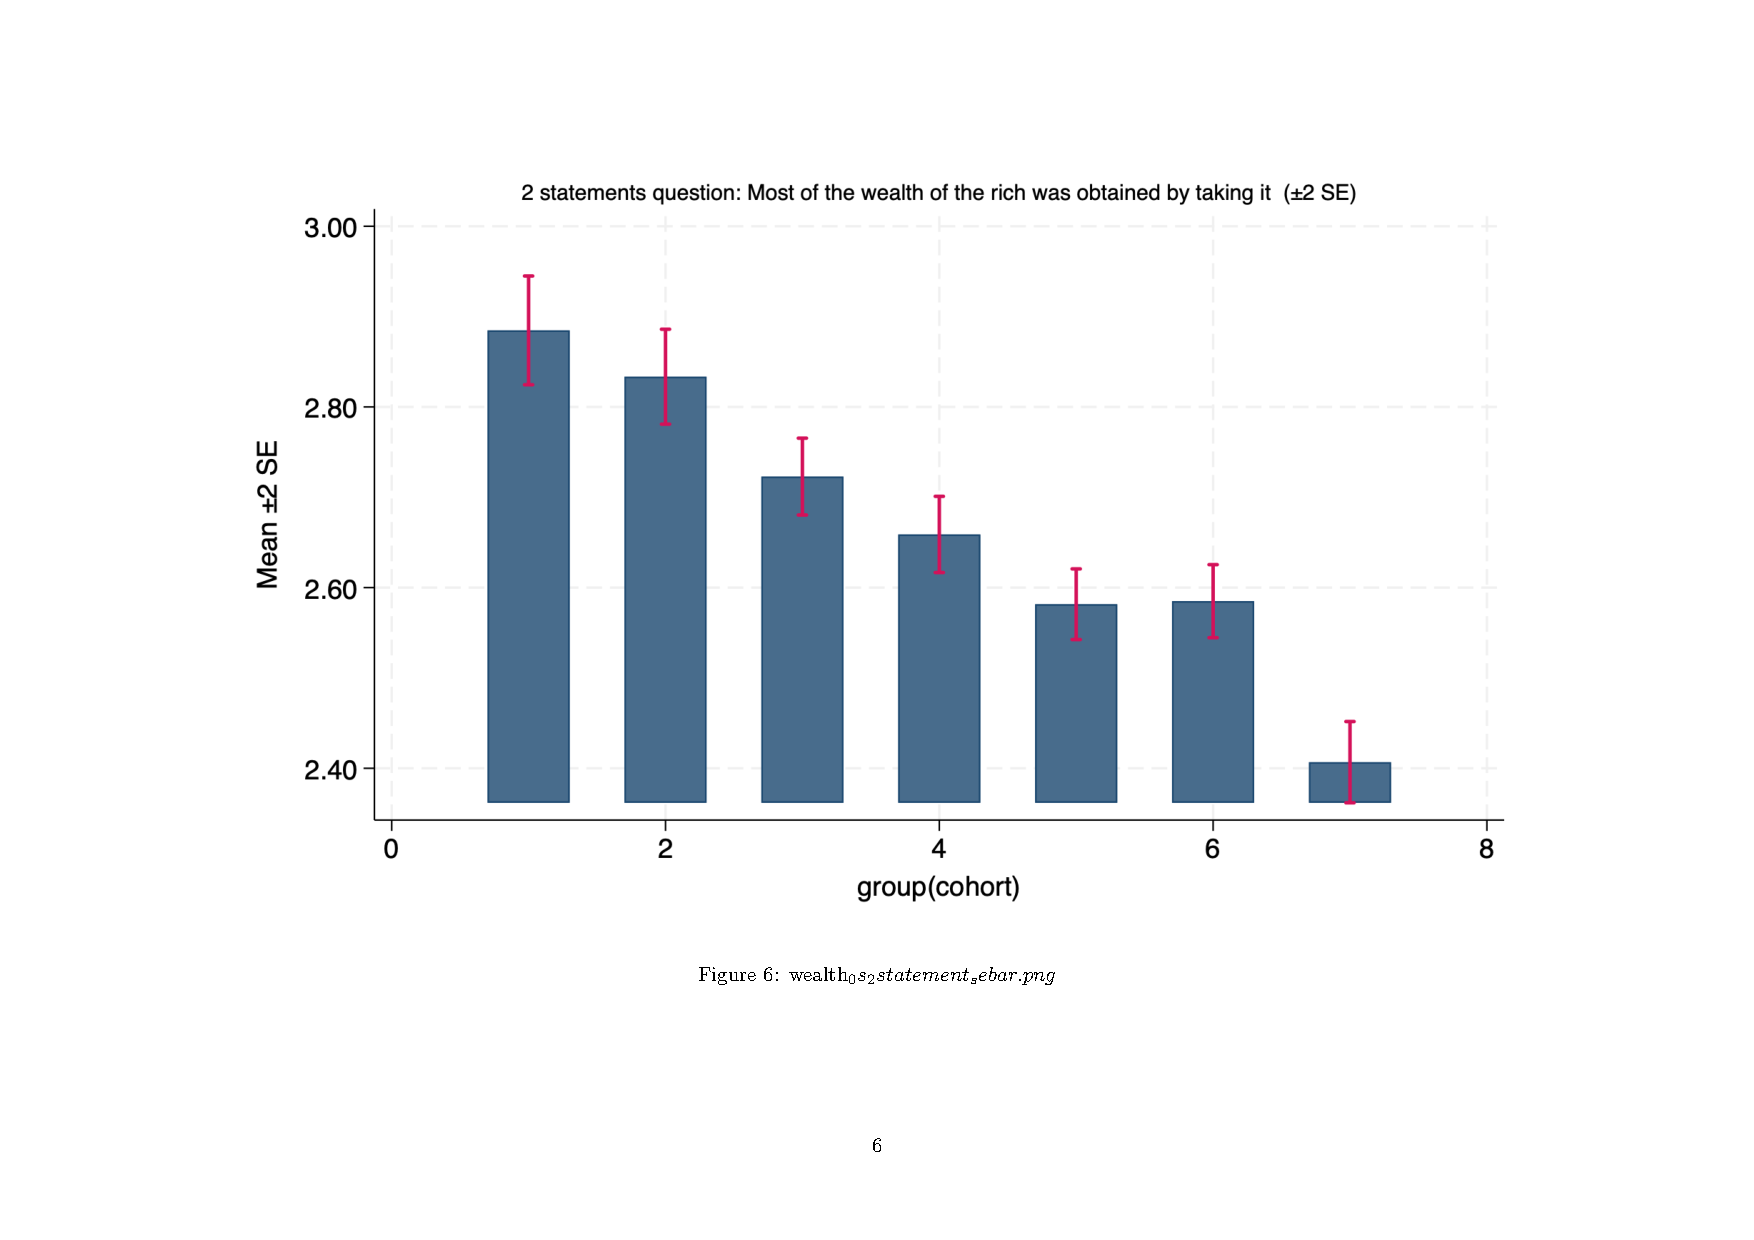
\includegraphics[width=\linewidth]{images/stantcheva2005_richbytaking.pdf}
    \end{subfigure}
\end{figure}
\begin{figure}[H]
    \centering
    \caption{Zero-sum ethnicity}
    \begin{subfigure}{.49\textwidth}
        \centering
        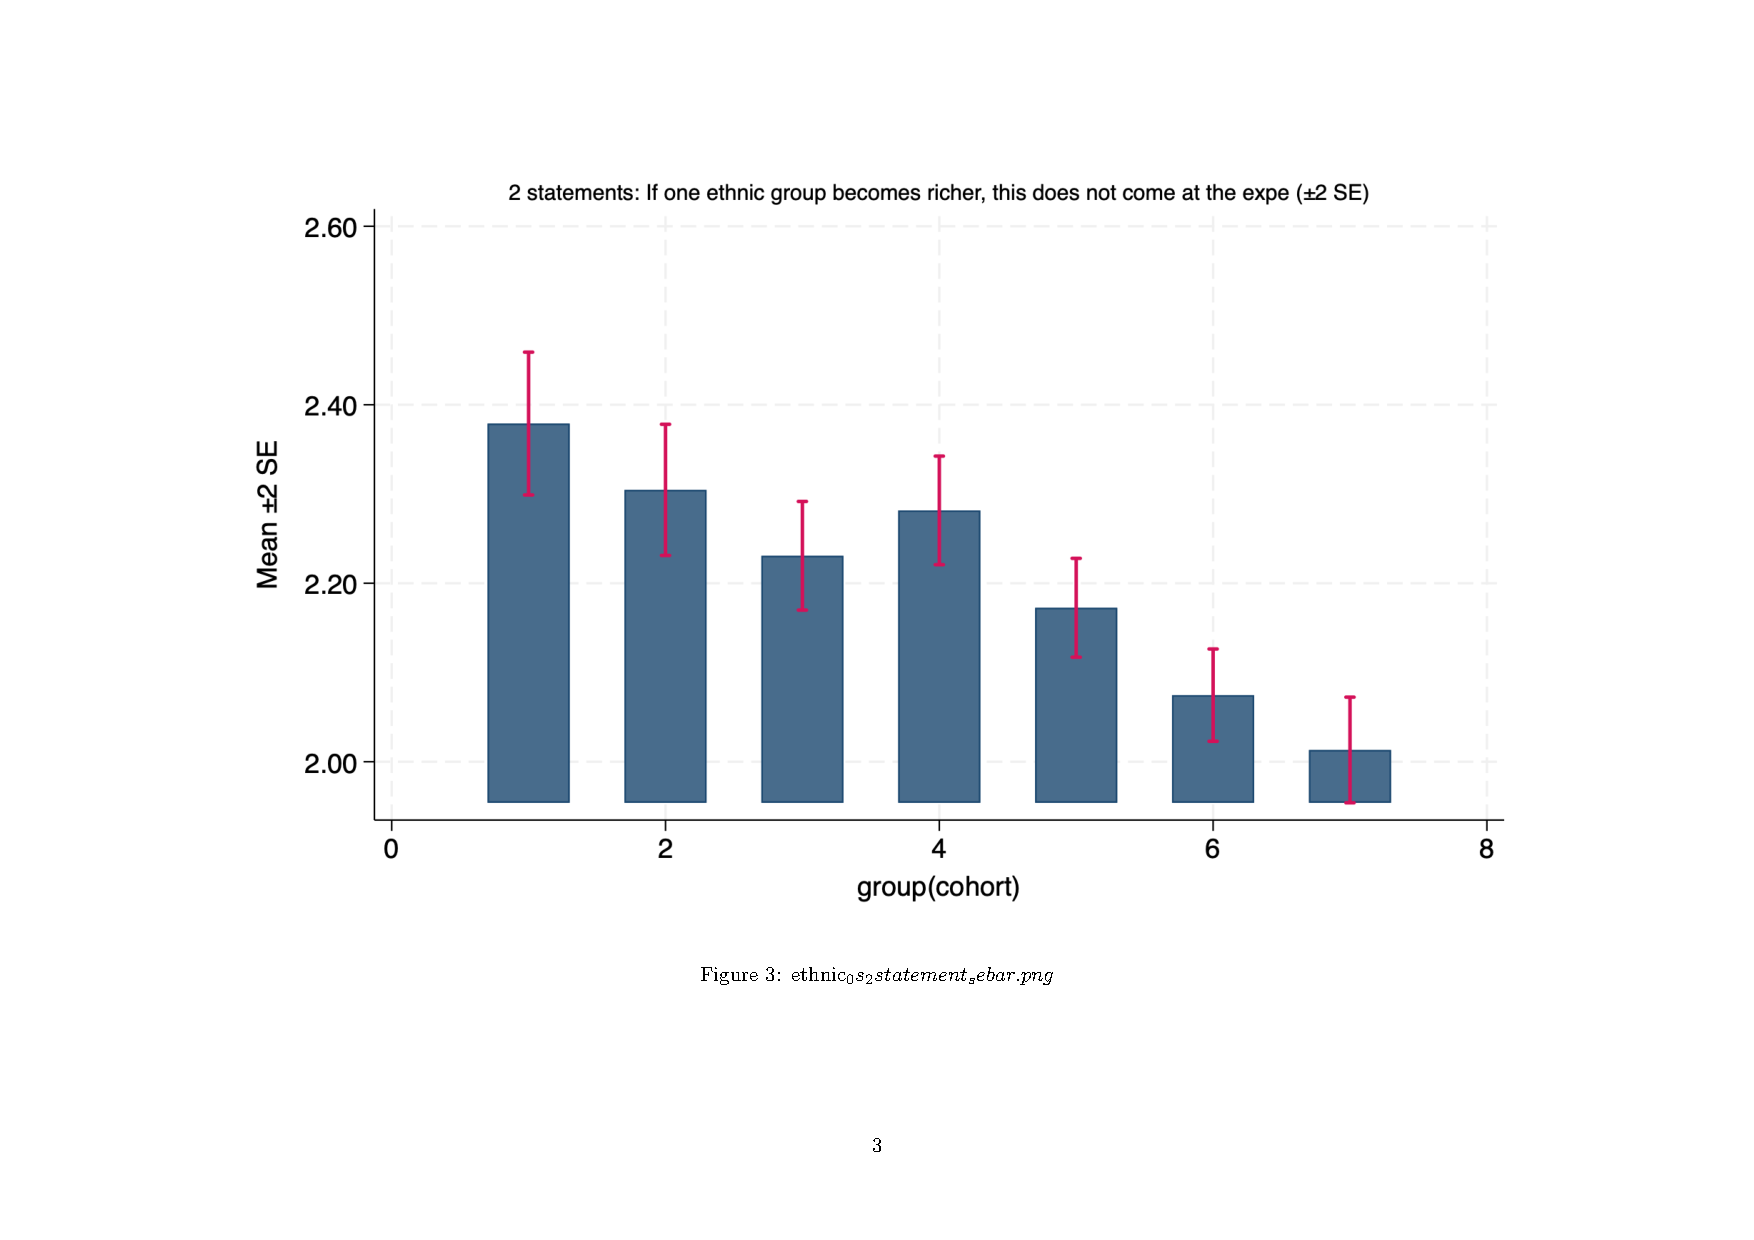
\includegraphics[width=\linewidth]{images/stantcheva2005_zerosumethnic.pdf}
    \end{subfigure}
\end{figure}
\begin{figure}[H]
    \centering
    \caption{Universalism}
    \begin{subfigure}{.49\textwidth}
        \centering
        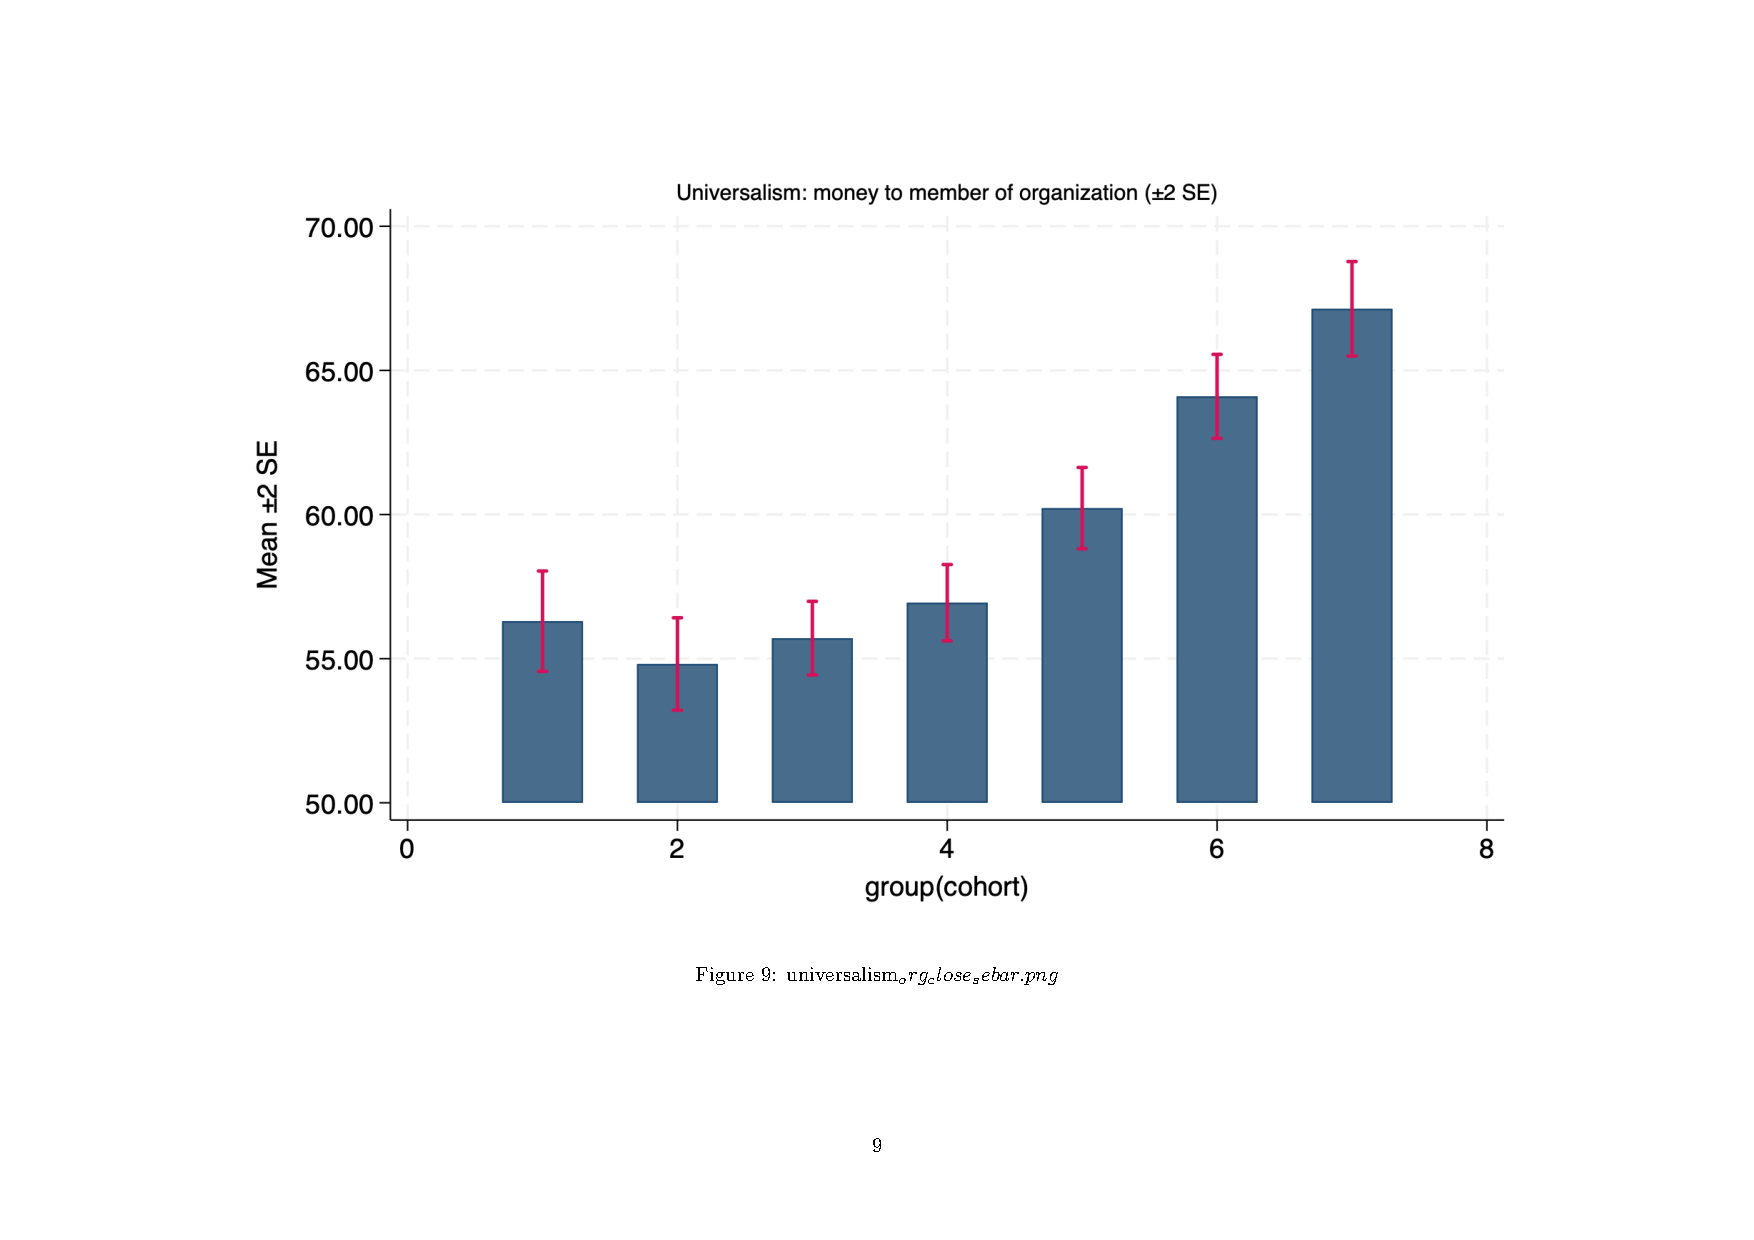
\includegraphics[width=\linewidth]{images/stantcheva2005_moneytomember.pdf}
    \end{subfigure}
    \begin{subfigure}{.49\textwidth}
        \centering
        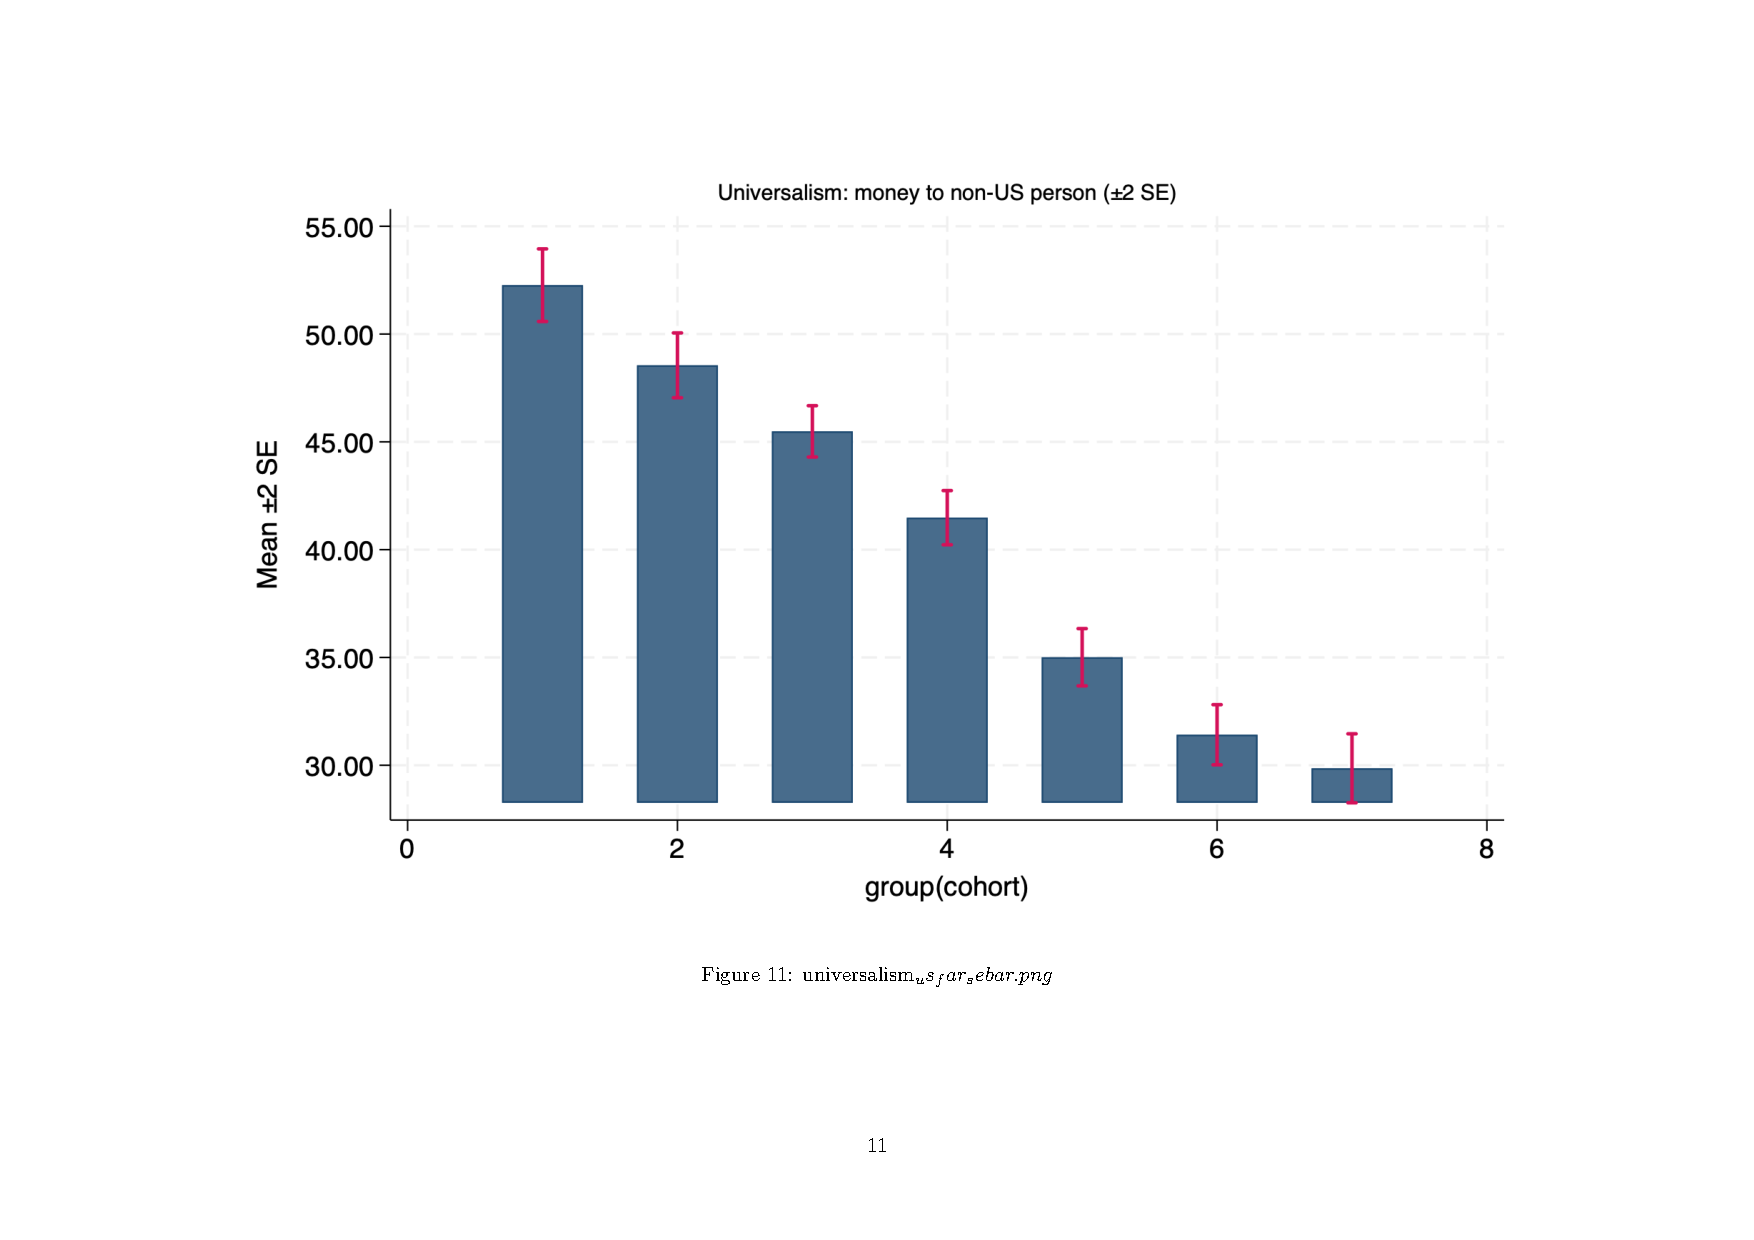
\includegraphics[width=\linewidth]{images/stantcheva2005_moneynonamerican.pdf}
    \end{subfigure}
\end{figure}




\end{document}
